\documentclass[a4paper, 11pt]{article}

\usepackage[T2A]{fontenc}
\usepackage[utf8]{inputenc}
\usepackage[english, russian]{babel}
\usepackage{amsmath}
\usepackage{graphicx}
\usepackage{subcaption}
\usepackage{float}
\usepackage{tabularx}

\usepackage{amsmath,booktabs}
\usepackage{array}
\righthyphenmin=2
\usepackage[left=20mm, top=15mm, right=15mm, bottom=15mm, nohead, footskip=10mm]{geometry} % настройки полей документа

\begin{document} 
% НАЧАЛО ДОКУМЕНТА	
\paragraph{Цель работы.}Исследование точностных свойств систем управления.
\paragraph{Исследование системы с астатизмом нулевого порядка.}Исследуемая система:\\
\large{$W(s)= \frac {2} {0.5s^2+s+2}$}

\begin{figure}[h]
    \center{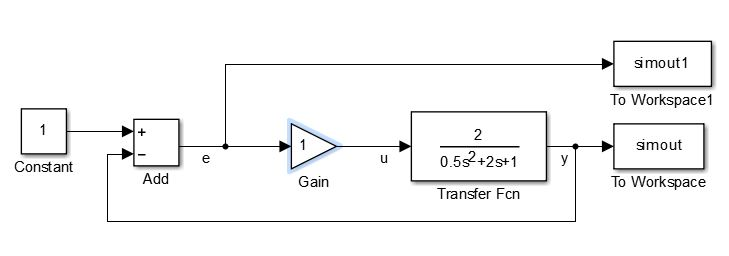
\includegraphics[width=1\linewidth]{1}}
    \caption{Система с астатизмом нулевого порядка.}
    \label{one}
\end{figure}

g(t) = A – стационарный режим работы. A = 2\\
%____________Это к1

Рассмотрим переходные процессы Y(t) и e(t) при К=1

\begin{figure}[h!]
    \center{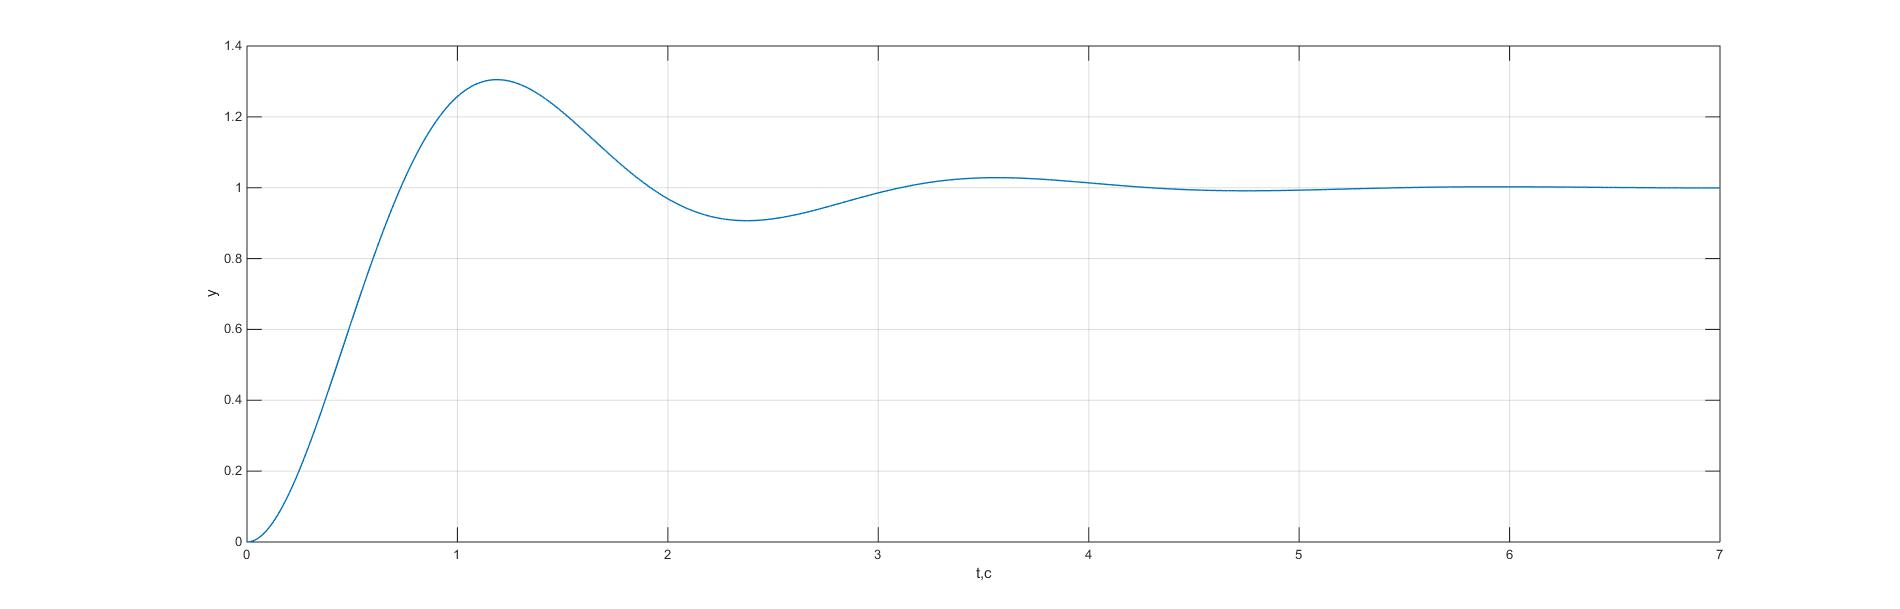
\includegraphics[width=1\linewidth]{1/1_y_a2_k1}}
    \caption{График переходного процесса при К=1}
    \label{two}
\end{figure}



\begin{figure}[h!]
    \center{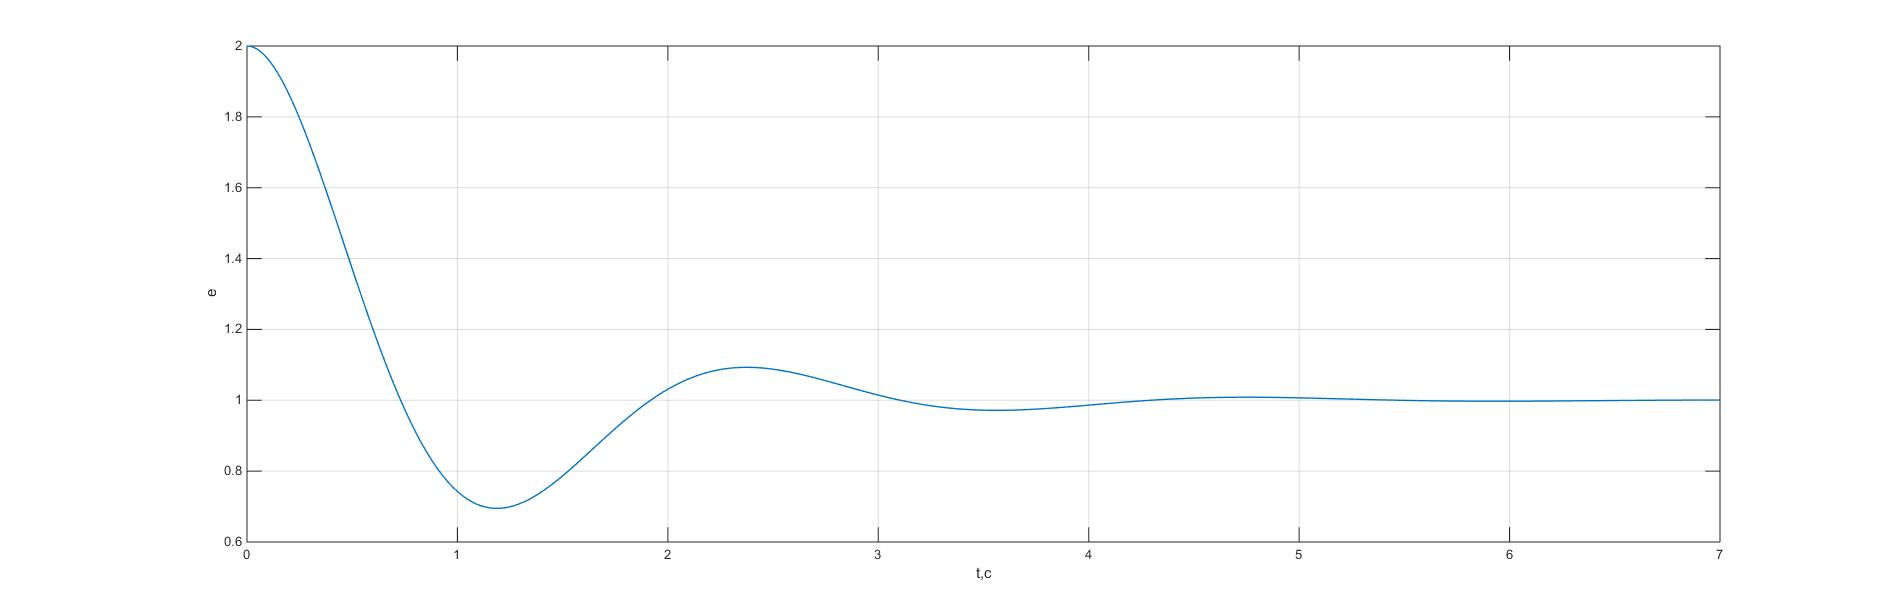
\includegraphics[width=1\linewidth]{1/1_e_a2_k1}}
    \caption{График ошибки переходного процесса при К=1}
    \label{tree}
\end{figure}

\newpage 

\large{$\epsilon=\frac {A}{1+k} = 2/(1+1) = 1$}

Из графика видно, что предельное значение установившейся ошибки \\ $\epsilon_y(t) = 1$. Это значение равно значению, полученному аналитическим расчетом.\\
%______________________Это к =5

Рассмотрим переходные процессы Y(t) и e(t) при К=5
\begin{figure}[h!]
    \center{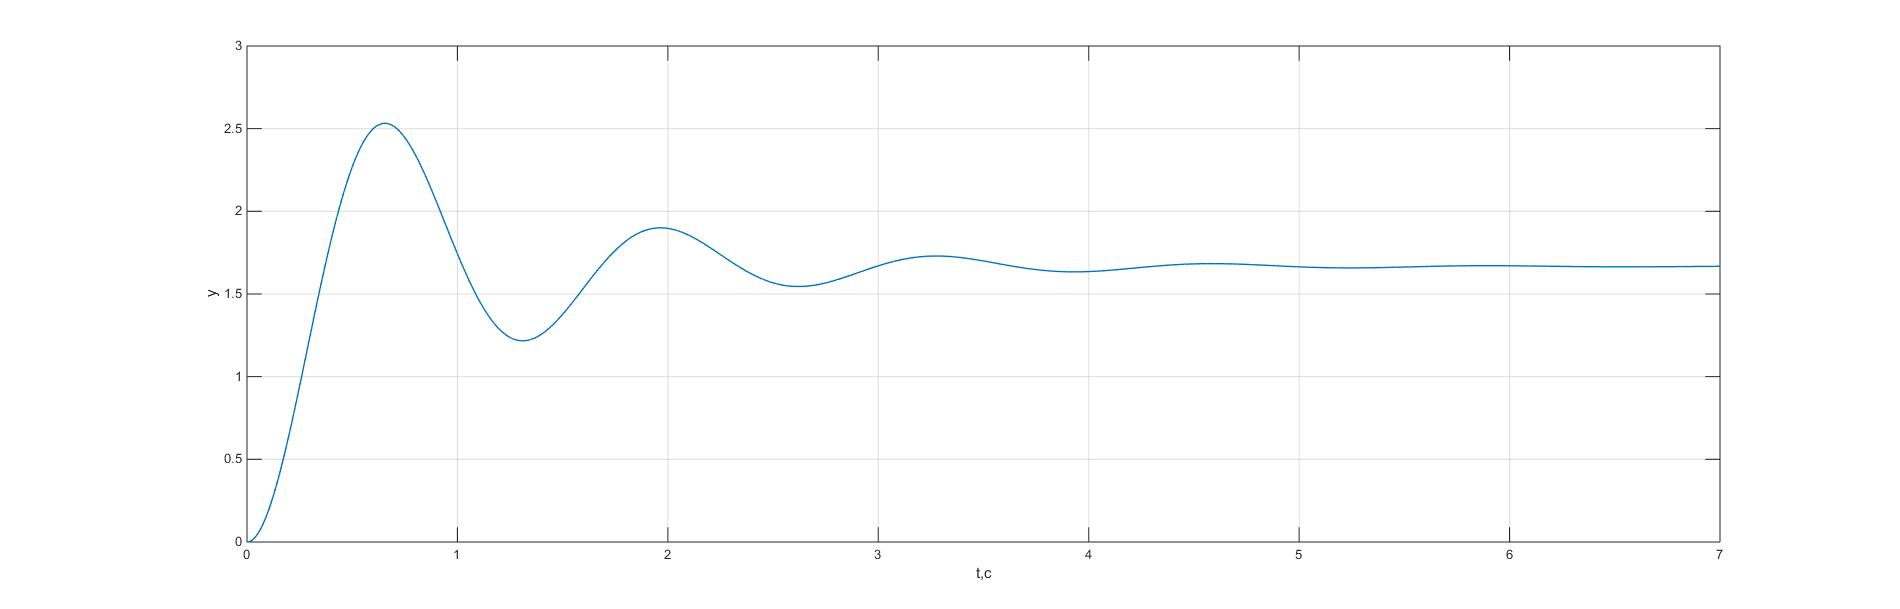
\includegraphics[width=1\linewidth]{1/1_y_a2_k5}}
    \caption{График переходного процесса при К=5}
    \label{four}
\end{figure}

\begin{figure}[h!]
    \center{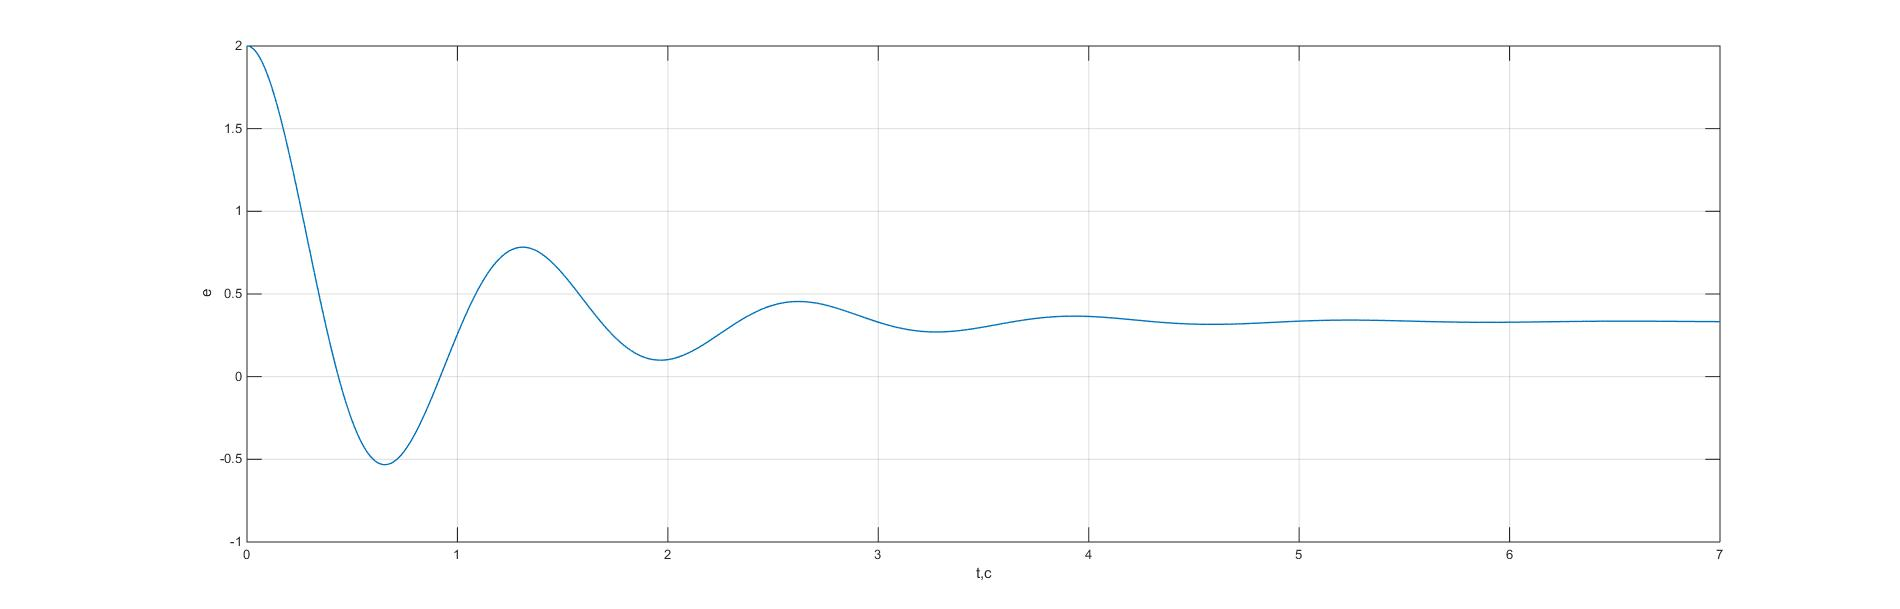
\includegraphics[width=1\linewidth]{1/1_e_a2_k5}}
    \caption{График ошибки переходного процесса при К=5}
    \label{tree}
\end{figure}

Из графика видно, что предельное значение установившейся ошибки $\epsilon_y(t)=0.33$.\\
Это значение подтверждается аналитиическим расчетом: $\epsilon=\frac {A}{1+k} = 2/(1+5) = 0.33$\\
%________________Это К10

Рассмотрим переходные процессы Y(t) и e(t) при К=10
\begin{figure}[h!]
    \center{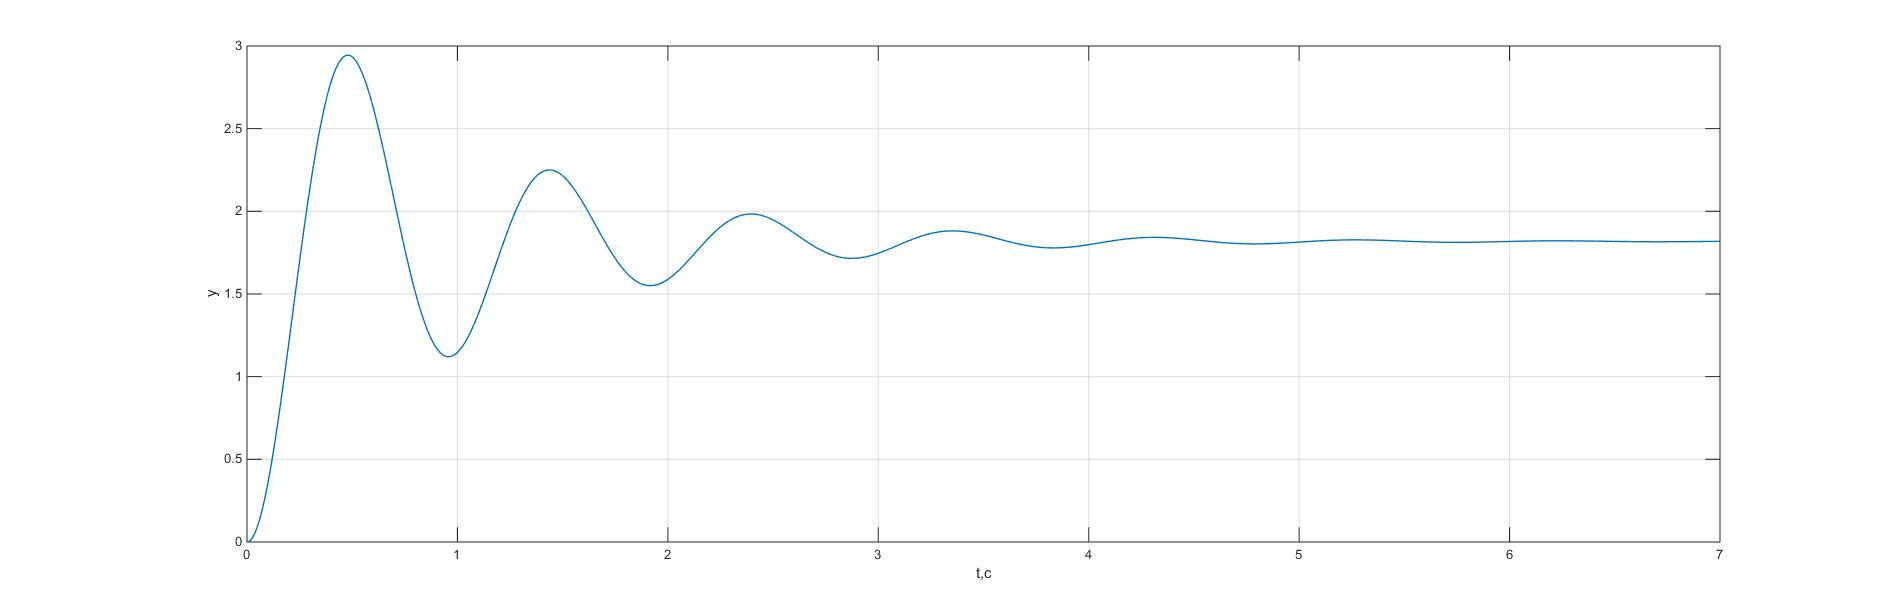
\includegraphics[width=1\linewidth]{1/1_y_a2_k10}}
    \caption{График переходного процесса К=10}
    \label{four}
\end{figure}

\newpage 

\begin{figure}[h!]
    \center{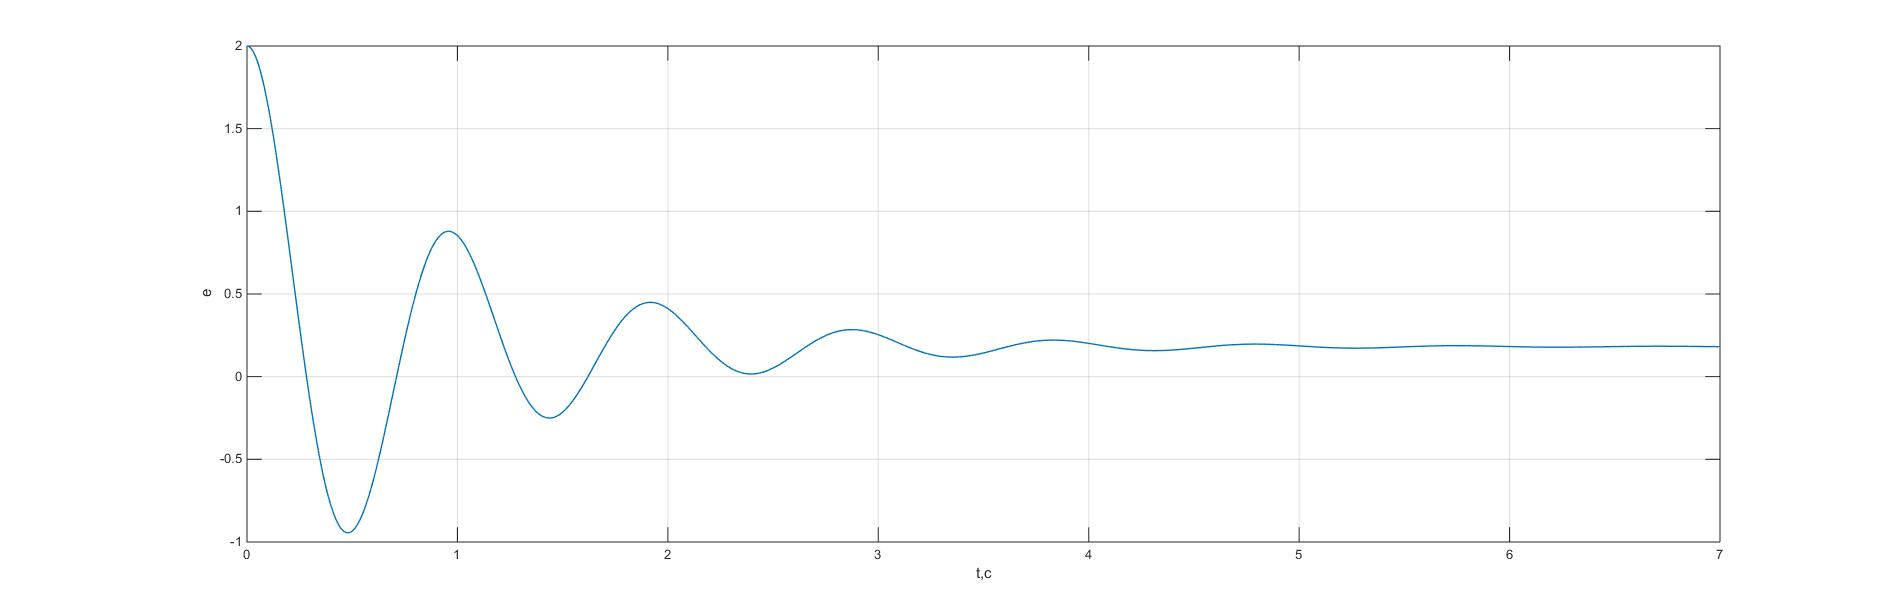
\includegraphics[width=1\linewidth]{1/1_e_a2_k10}}
    \caption{График ошибки переходного процесса при К=10}
    \label{tree}
\end{figure}

\normalsize{Из графика видно, что предельное значение установившейся ошибки $\epsilon_y(t)=0.2$.
Это значение очень близко к значению, полученному аналитическим расчетом: $\epsilon=\frac {A}{1+k} = 2/(1+10) = 0.18$}

\begin{table}[h]
    \begin{center}
    \begin{tabular}{|c|c|c|c|}
    \hline
         K & 1 & 5 & 10 \\
         \hline
         $\epsilon$ & 1 & 0.33 & 0.18 \\
    \hline     
    \end{tabular}
    \caption{Зависимость коэффициента от ошибки}
    \label{tab:my_label}
    \end{center}
\end{table}

%_______________ПРИ g(t)=Vt
б) g(t) = Vt – движение с постоянной скоростью. V = 2\\

Рассмотрим переходные процессы Y(t) и e(t) при К=1

\begin{figure}[h!]
    \center{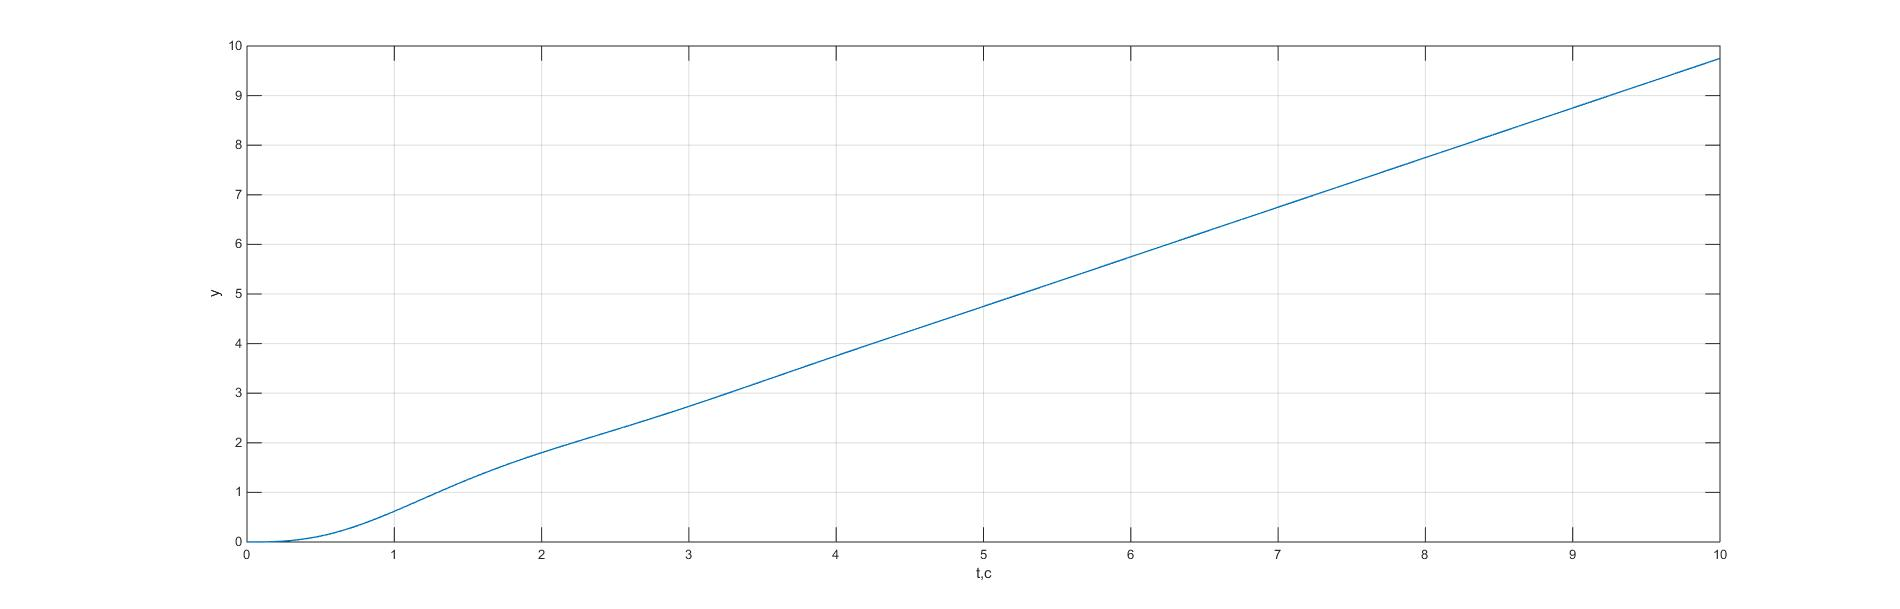
\includegraphics[width=1\linewidth]{1/7}}
    \caption{График переходного процесса при К=1}
    \label{four}
\end{figure}

\begin{figure}[h!]
    \center{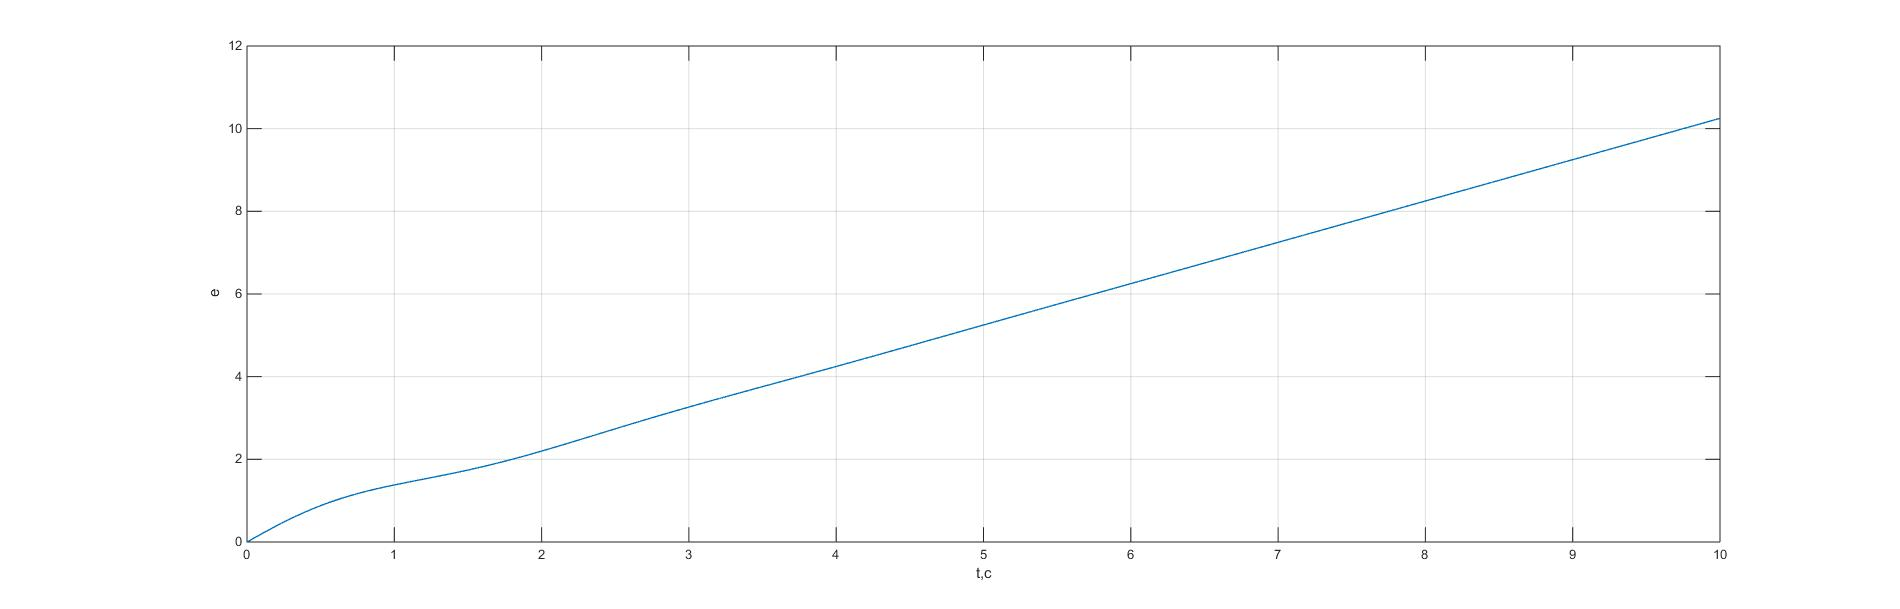
\includegraphics[width=1\linewidth]{1/8}}
    \caption{График ошибки переходного процесса при К=1}
    \label{tree}
\end{figure}

\newpage

Рассмотрим переходные процессы Y(t) и e(t) при К=5

\begin{figure}[h!]
    \center{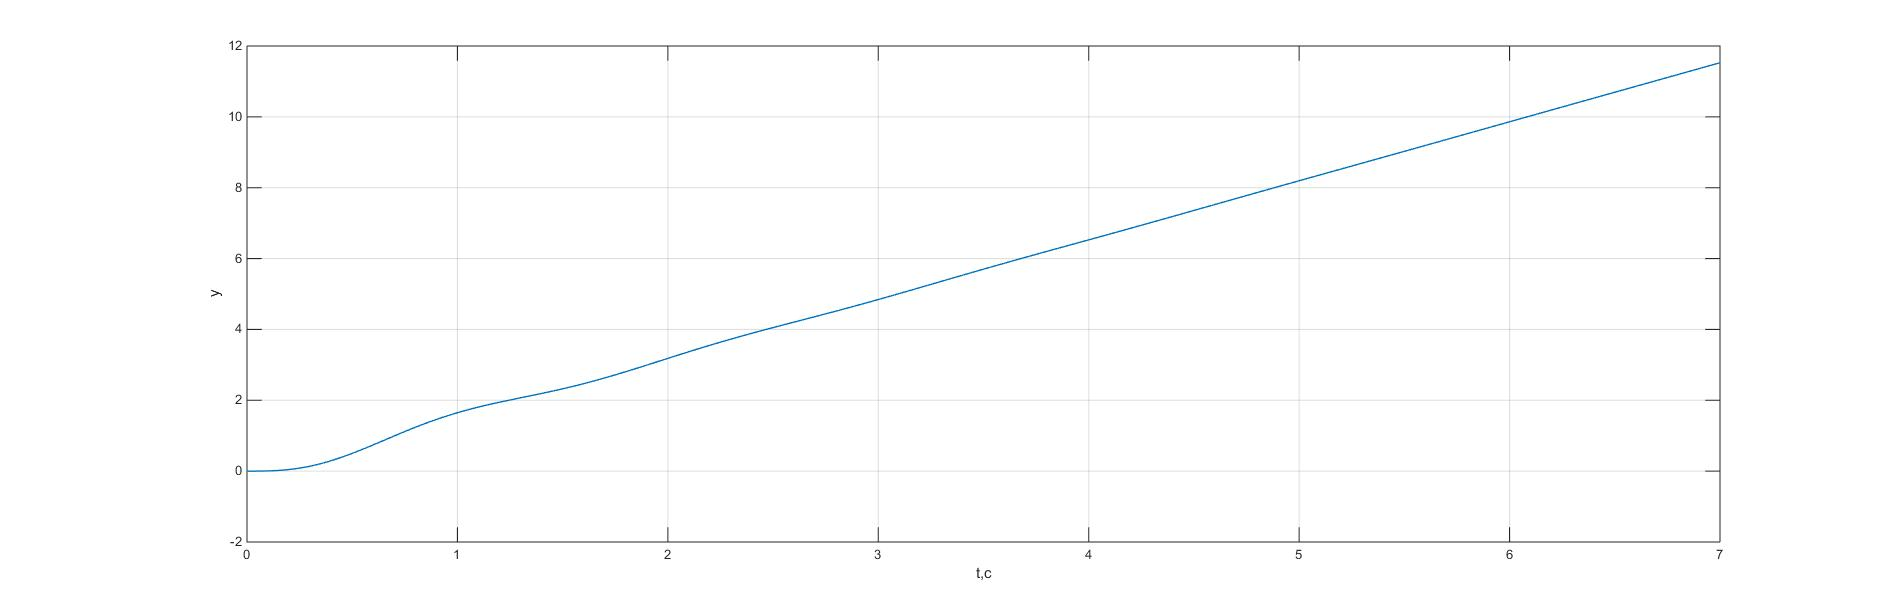
\includegraphics[width=1\linewidth]{1/9}}
    \caption{График переходного процесса при К=5}
    \label{four}
\end{figure}

\begin{figure}[h!]
    \center{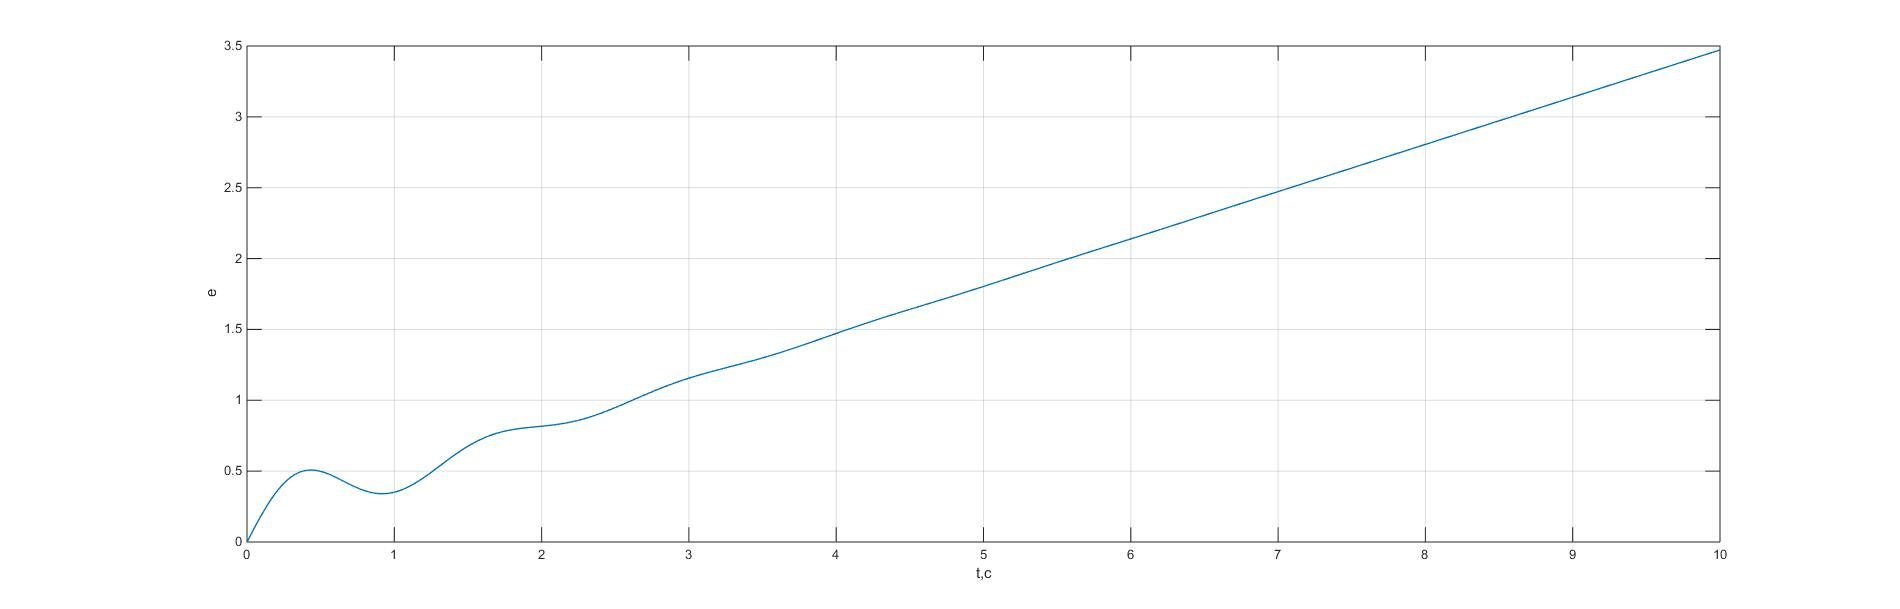
\includegraphics[width=1\linewidth]{1/10}}
    \caption{График ошибки переходного процесса при К=5}
    \label{tree}
\end{figure}

Рассмотрим переходные процессы Y(t) и e(t) при К=10

\begin{figure}[h!]
    \center{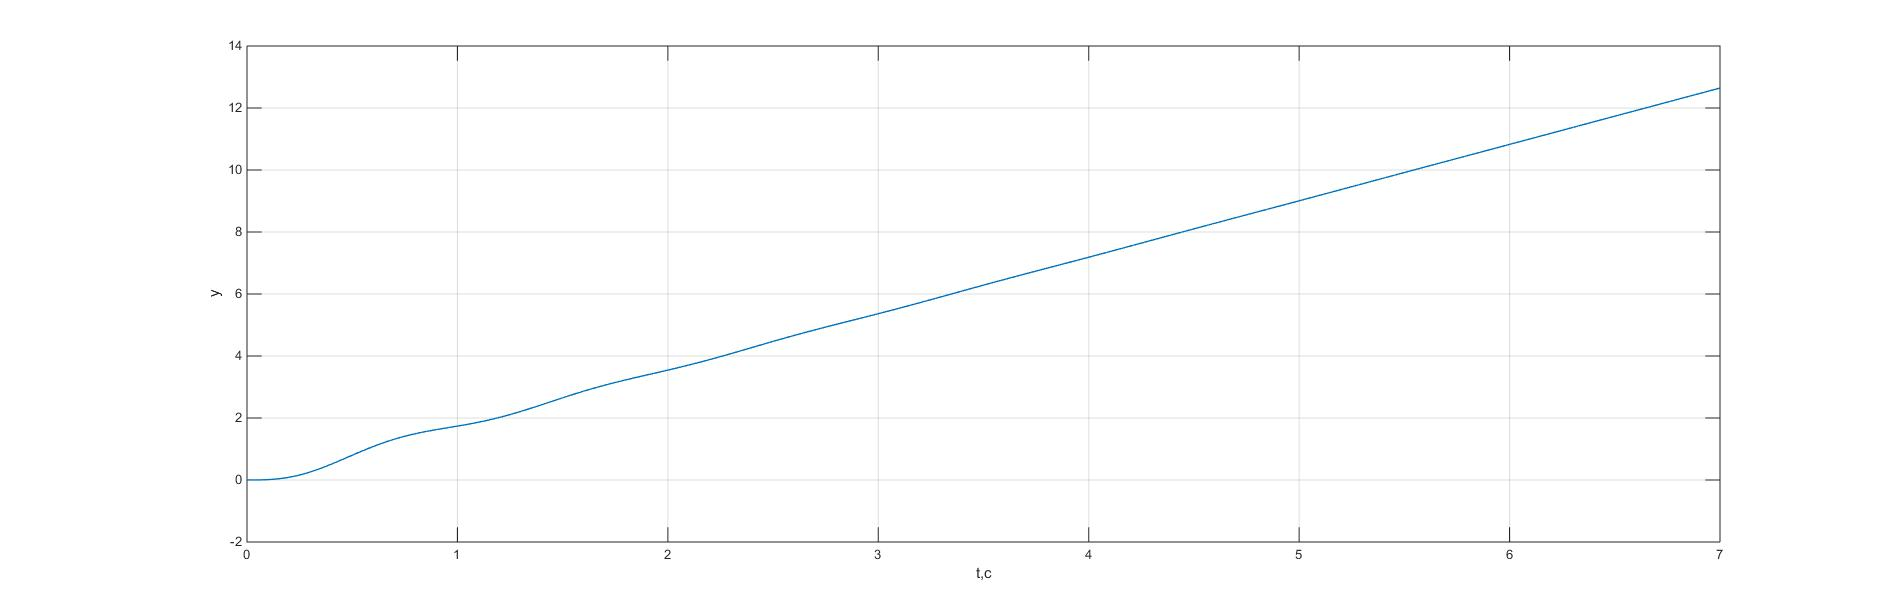
\includegraphics[width=1\linewidth]{1/11}}
    \caption{График переходного процесса при К=10}
    \label{four}
\end{figure}

\newpage

\begin{figure}[h!]
    \center{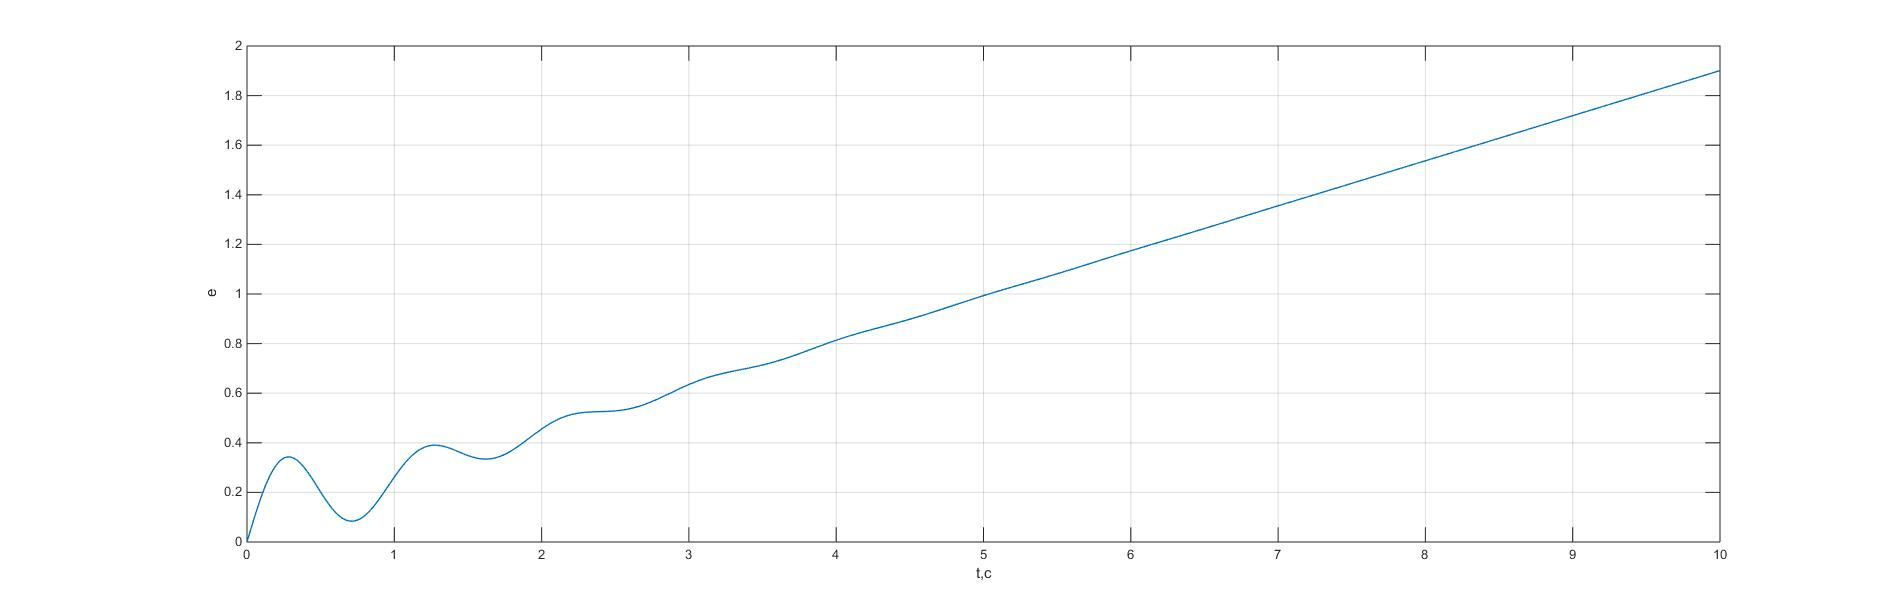
\includegraphics[width=1\linewidth]{1/12}}
    \caption{График ошибки переходного процесса при К=10}
    \label{tree}
\end{figure}

$\epsilon_y(t)=\lim_{s\to0}s\frac{1}{1+W(s)}\frac{V}{s^2}=\lim_{s\to0}\frac{1}{1+k}\frac{V}{s}=\infty$

Во всех случаях $\epsilon\to\infty$ \\

\textbf{Вывод.} СУ с нулевым порядком астатизма неспособна отработать изменяющееся задающее воздействие без ошибок, причем с течением времени ошибка увеличивается.
%___________________ВТОРАЯ ЧАСТЬ____________________
\newpage
\paragraph{Исследование системы с астатизмом первого порядка.}

Исследуемая система: \large{$W(s)=\frac{s+2}{0.5s^2+s+2}$}


\begin{figure}[h!]
    \center{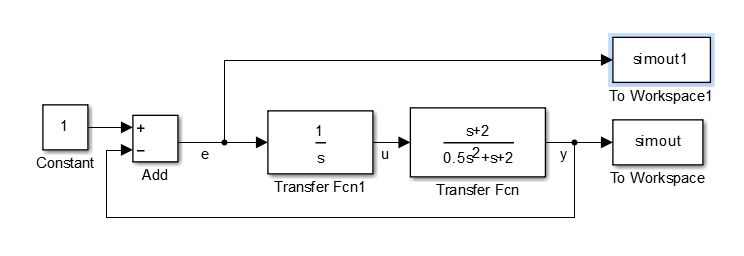
\includegraphics[width=1\linewidth]{2}}
    \caption{Система с астатизмом первого порядка.}
    \label{one}
\end{figure}
%___________Поехали а

g(t) = A – стационарный режим работы. A = 2.\\

Рассмотрим переходные процессы Y(t) и e(t) при К=1

\begin{figure}[h!]
    \center{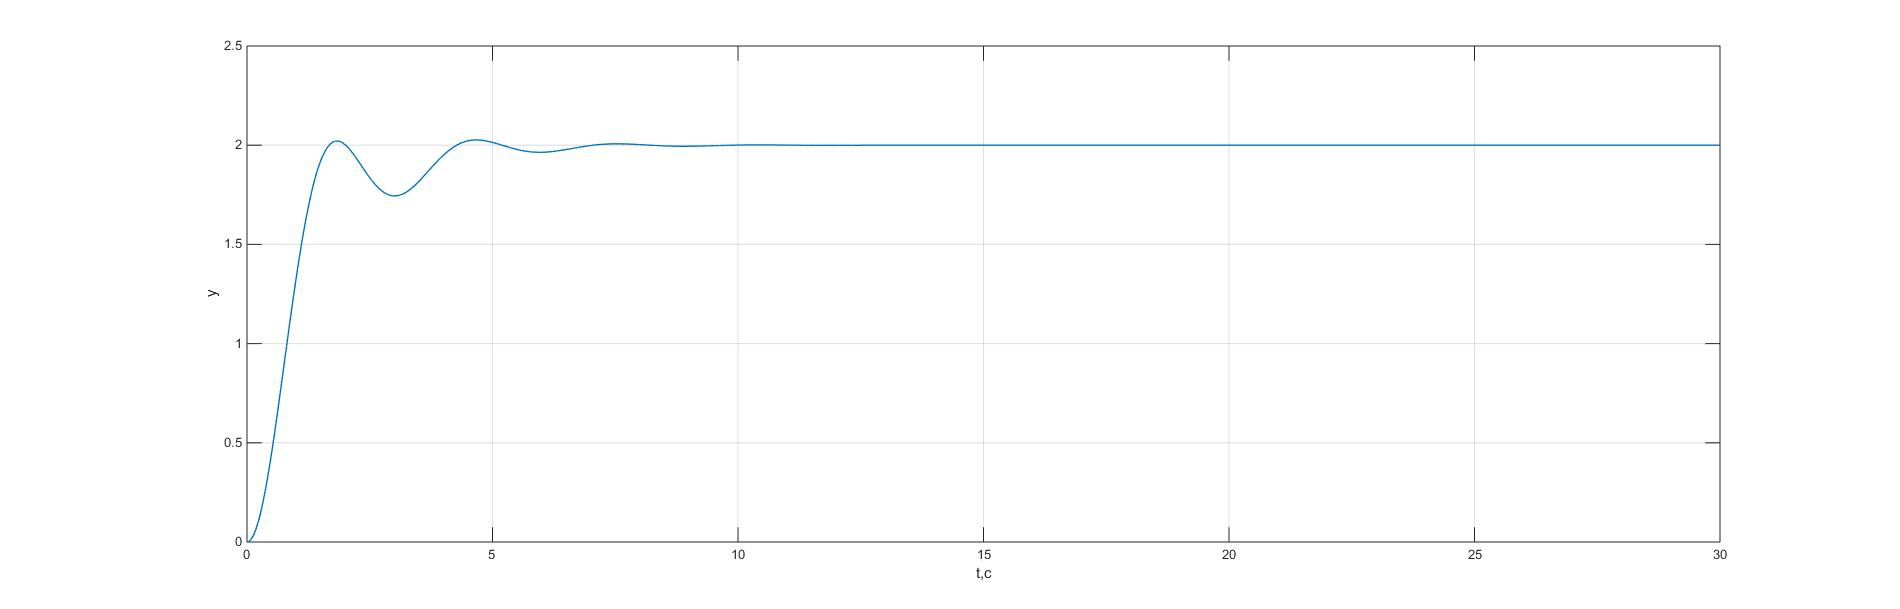
\includegraphics[width=1\linewidth]{2/2_13}}
    \caption{График переходного процесса при К=1}
    \label{two}
\end{figure}
\begin{figure}[h!]
    \center{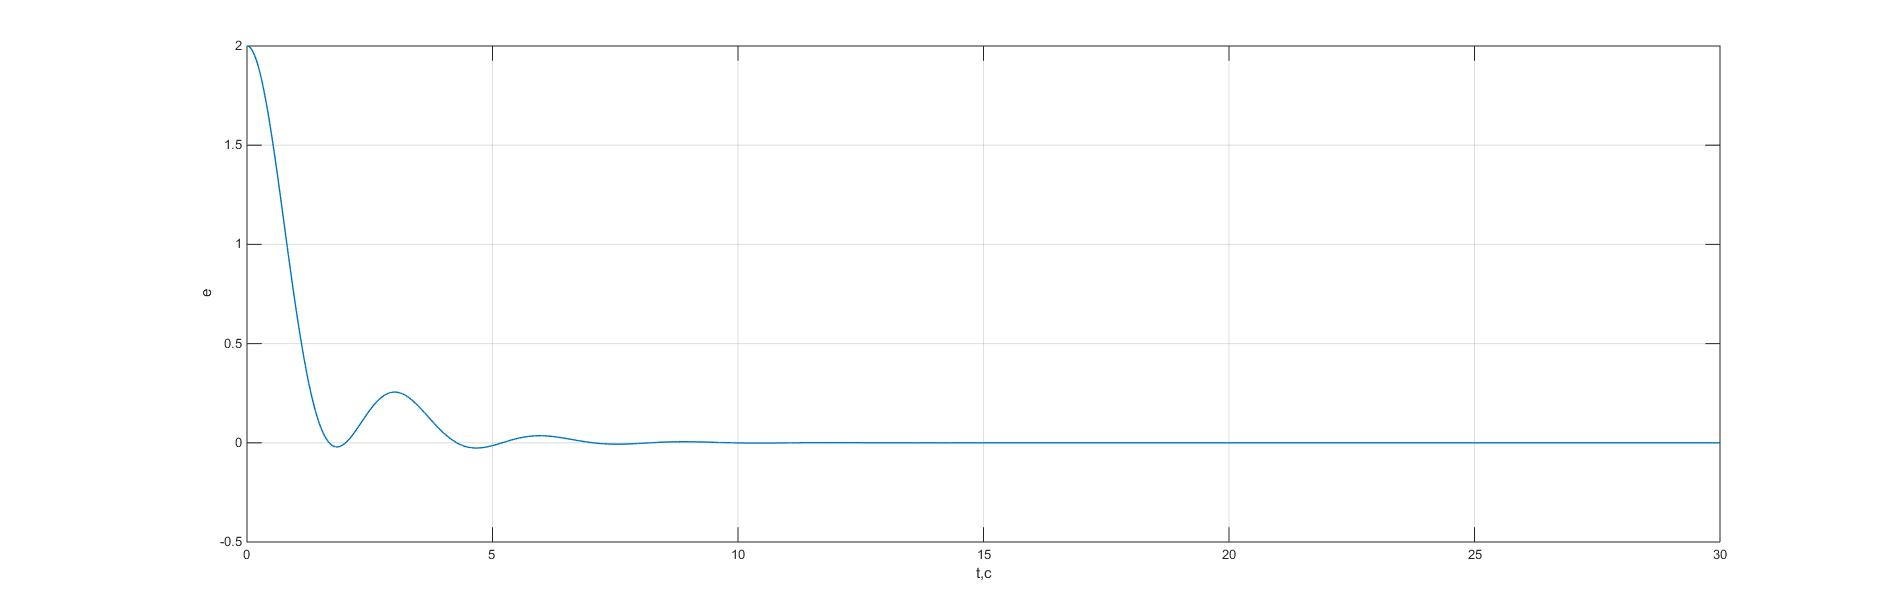
\includegraphics[width=1\linewidth]{2/14}}
    \caption{График ошибки переходного процесса при К=1}
    \label{tree}
\end{figure}

\newpage

Из графика видно, что предельное значение установившейся ошибки $\epsilon_y(t)=0$. Это значение подтверждается аналитическим расчетом: $\epsilon_y(t)=\lim_{s\to0}\frac{s}{s+k}A=0$\\

Рассмотрим переходные процессы Y(t) и e(t) при К=5

\begin{figure}[h!]
    \center{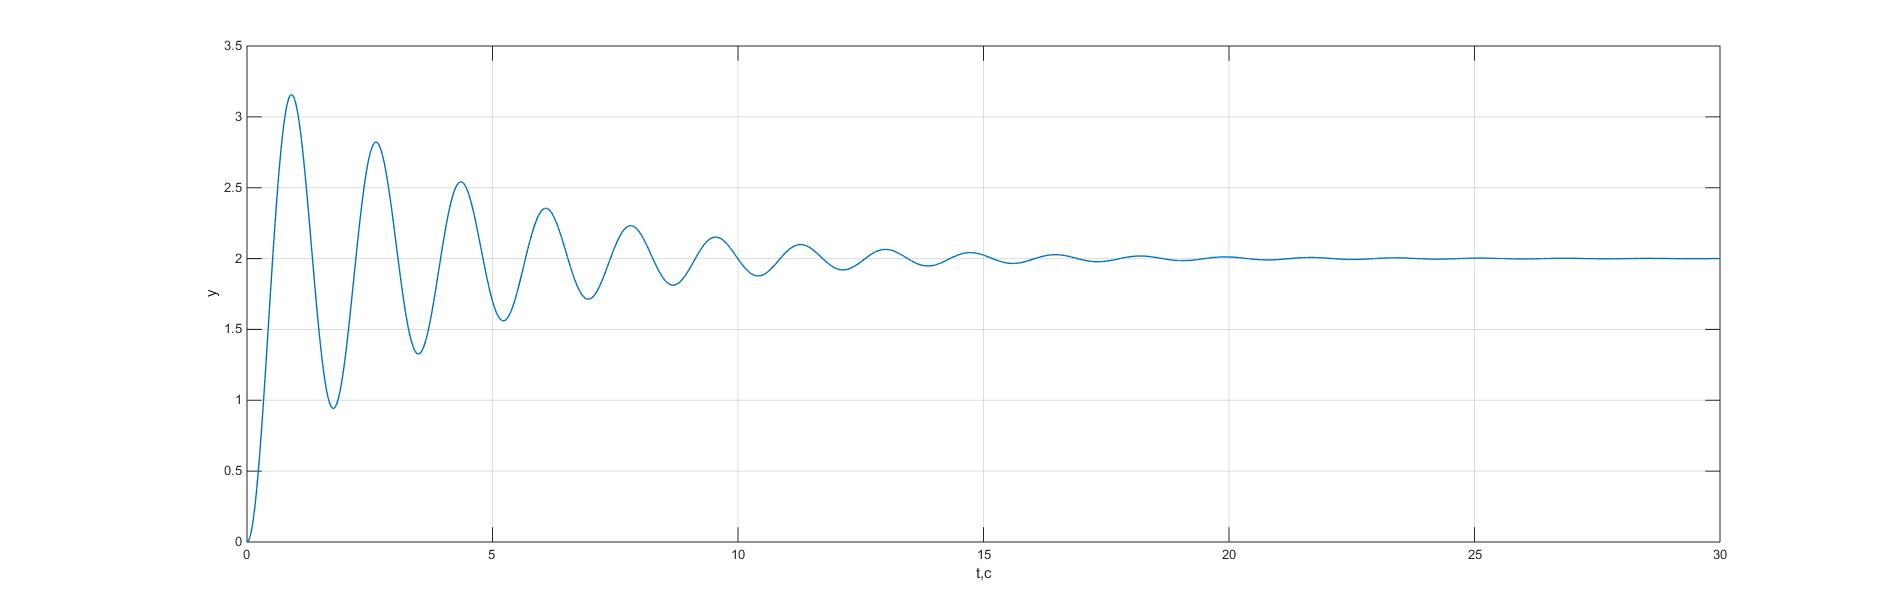
\includegraphics[width=1\linewidth]{2/15}}
    \caption{График переходного процесса при К=5}
    \label{two}
\end{figure}
\begin{figure}[h!]
    \center{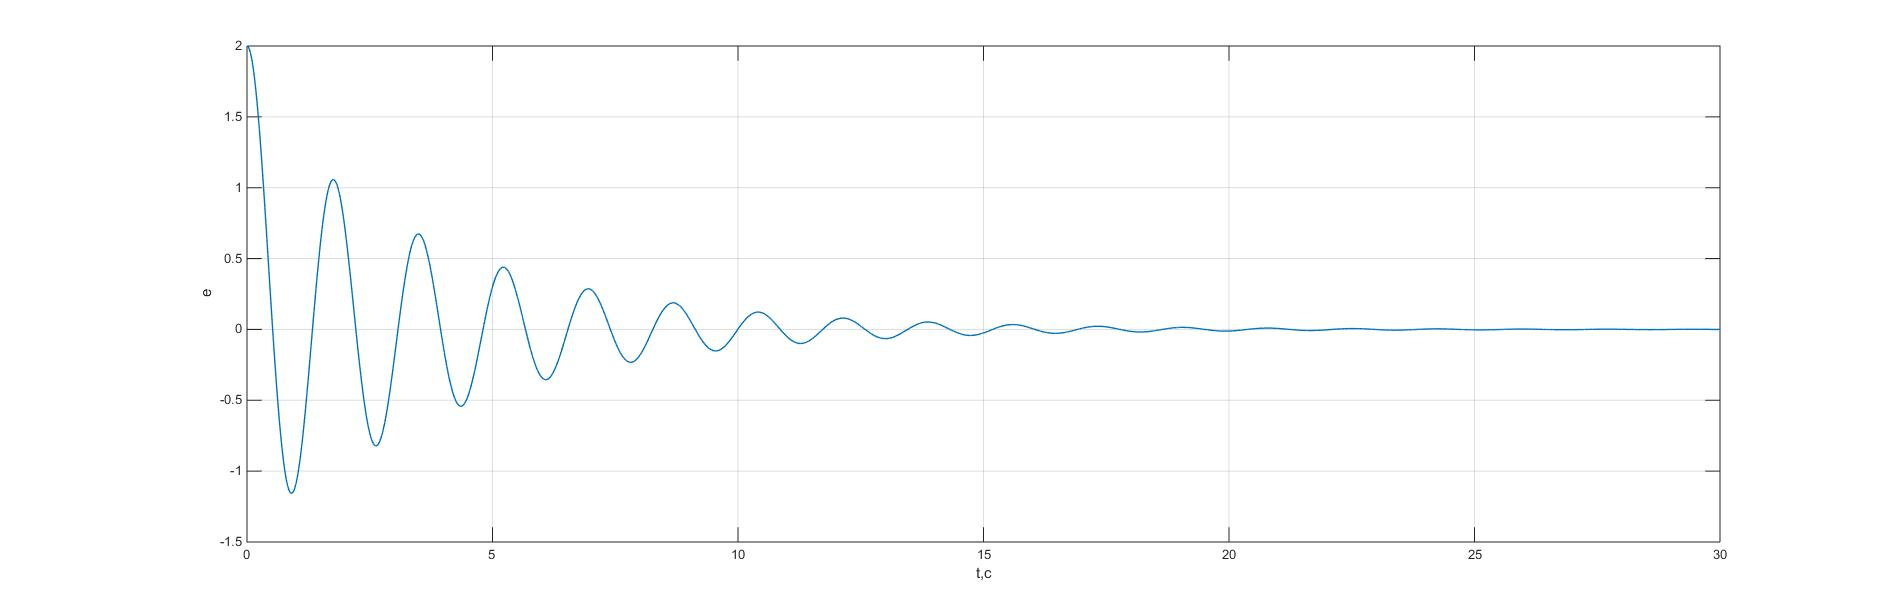
\includegraphics[width=1\linewidth]{2/16_e_k5_a2}}
    \caption{График ошибки переходного процесса при К=5}
    \label{tree}
\end{figure}

$\epsilon_y(t)=0$\\

Рассмотрим переходные процессы Y(t) и e(t) при К=10

\begin{figure}[h!]
    \center{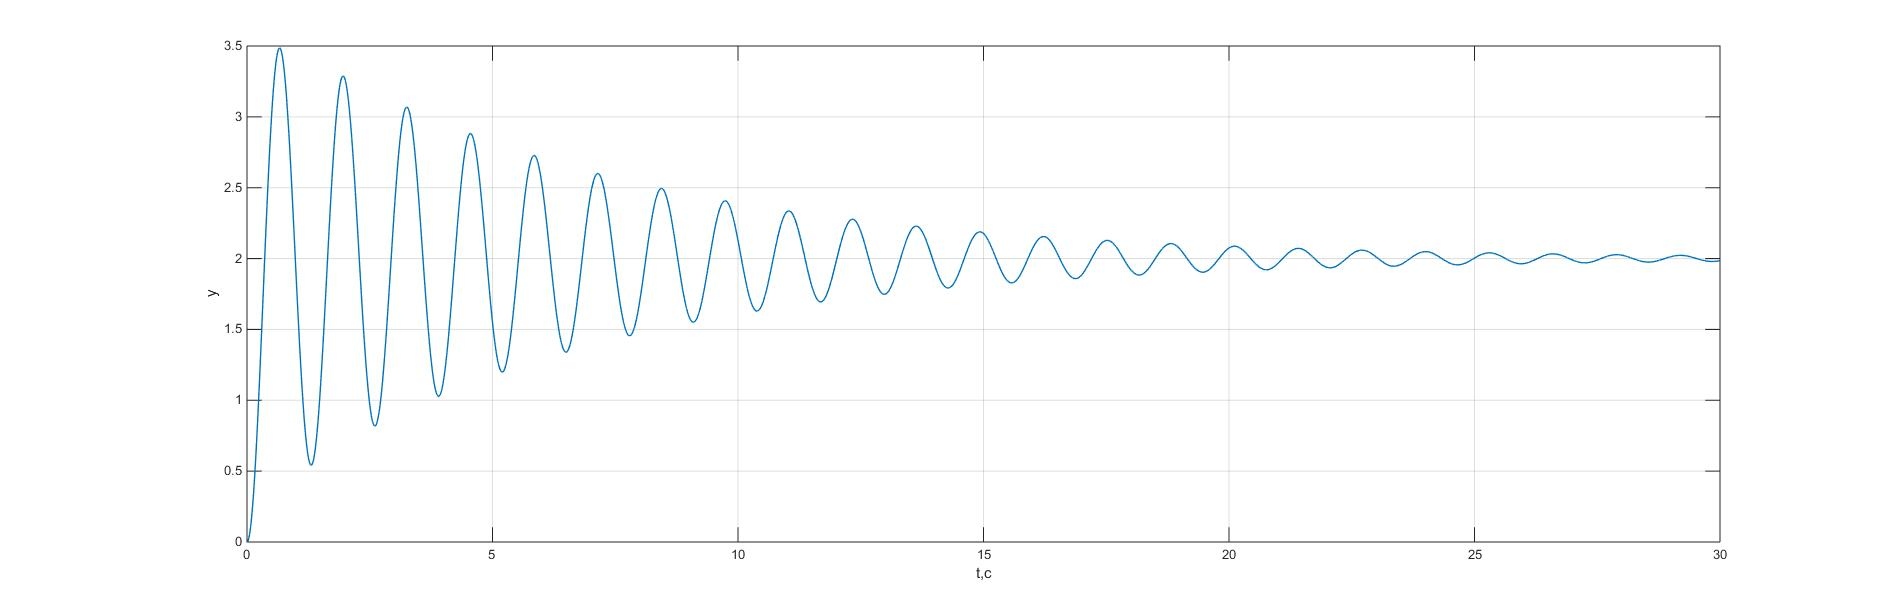
\includegraphics[width=1\linewidth]{2/17_y_k10_a2}}
    \caption{График переходного процесса при К=10}
    \label{two}
\end{figure}

\newpage

\begin{figure}[h!]
    \center{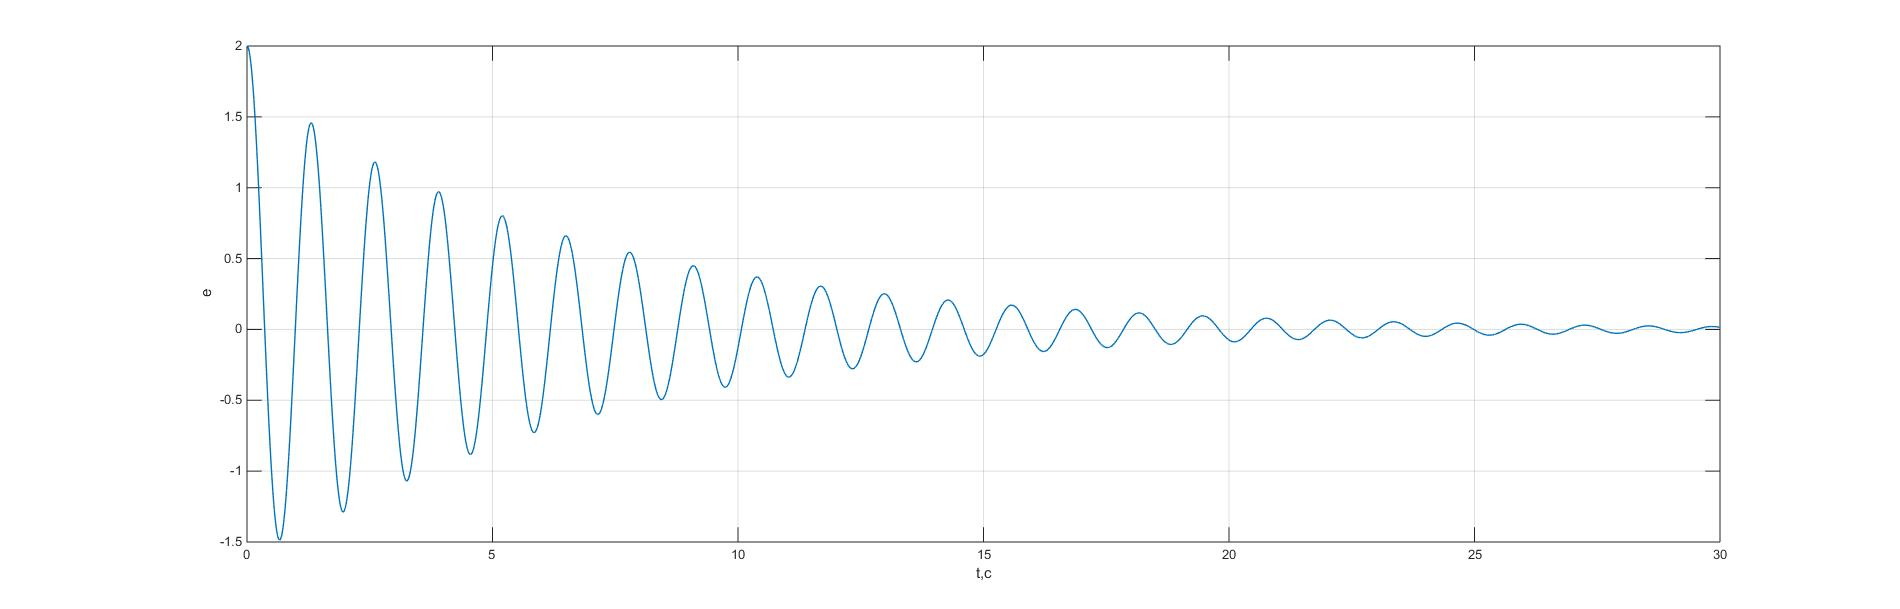
\includegraphics[width=1\linewidth]{2/18_e_k10_a2}}
    \caption{График ошибки переходного процесса при К=10}
    \label{tree}
\end{figure}

$\epsilon_y(t)=0$\\

Во всех трех случаях $\epsilon = 0$\\

\textbf{Вывод.} СУ с астатизмом первого порядка (и выше) отрабатывает постоянное задающее воздействие с нулевой установившейся ошибкой.\\


%___________________Б-часть второго параграфа
g(t)=Vt – движение с постоянной скоростью.  $V = 2; \epsilon=\frac{V}{K}$\\

Рассмотрим переходные процессы Y(t) и e(t) при К=1

\begin{figure}[h!]
    \center{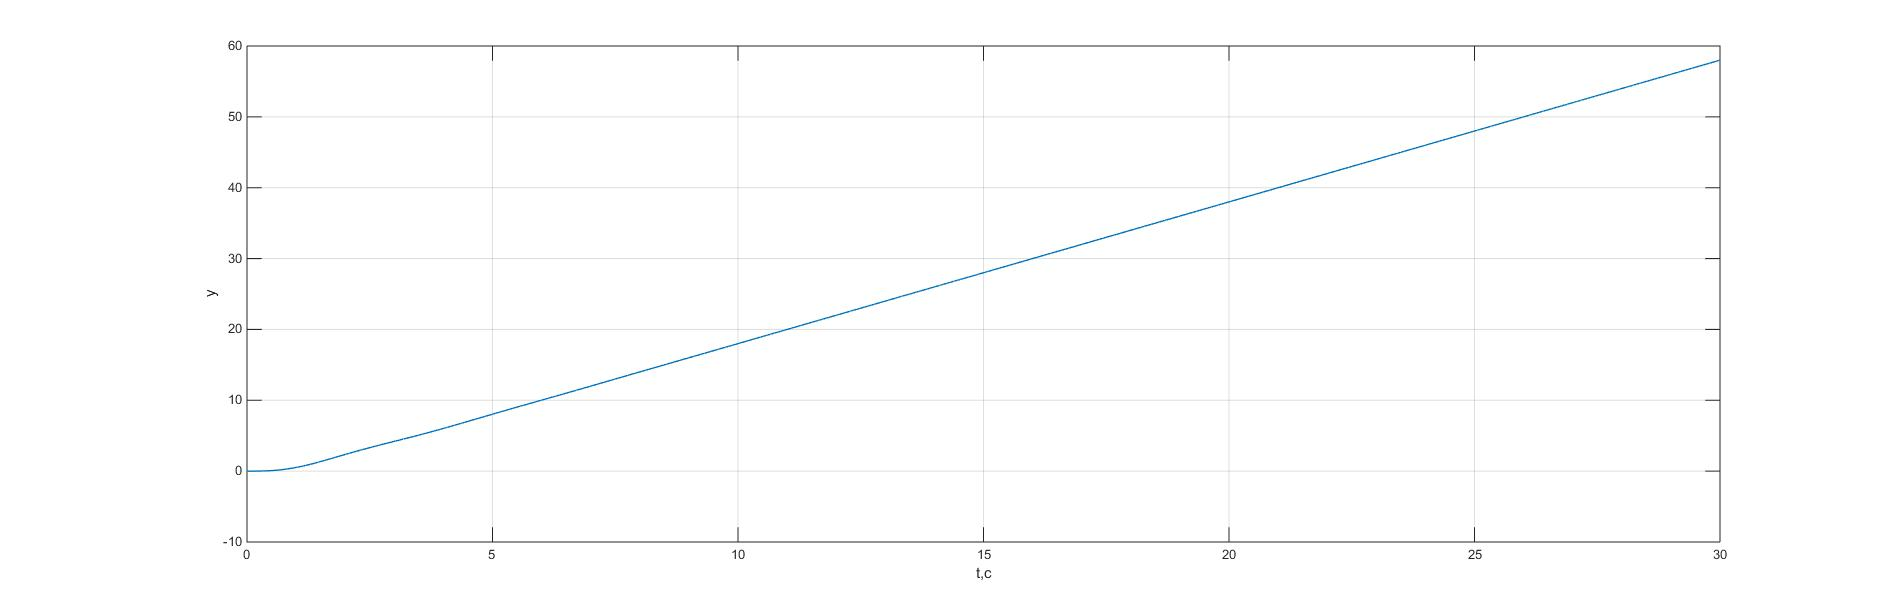
\includegraphics[width=1\linewidth]{2/19_y_k1_2t}}
    \caption{График переходного процесса при К=1}
    \label{two}
\end{figure}

\begin{figure}[h!]
    \center{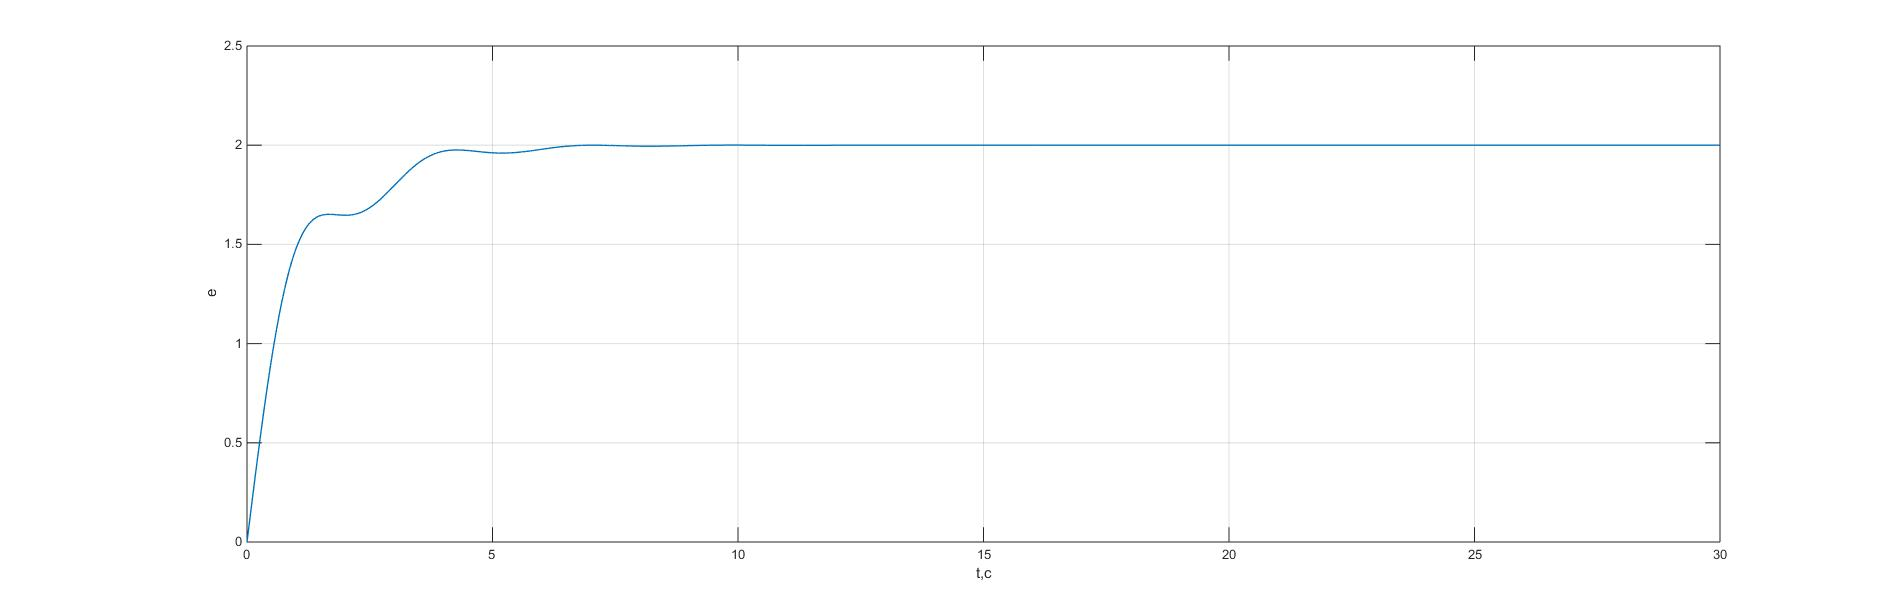
\includegraphics[width=1\linewidth]{2/20_e_k1_2t}}
    \caption{График ошибки переходного процесса при К=1}
    \label{tree}
\end{figure}

\newpage

Из графика видно, что предельное значение установившейся ошибки $\epsilon_y(t)=2$. Это значение подтверждается аналитическим расчетом: $\epsilon_y(t)=\lim_{s\to0}\frac{s}{s+k}V=\frac{V}{k}=2$\\

Рассмотрим переходные процессы Y(t) и e(t) при К=5

\begin{figure}[h!]
    \center{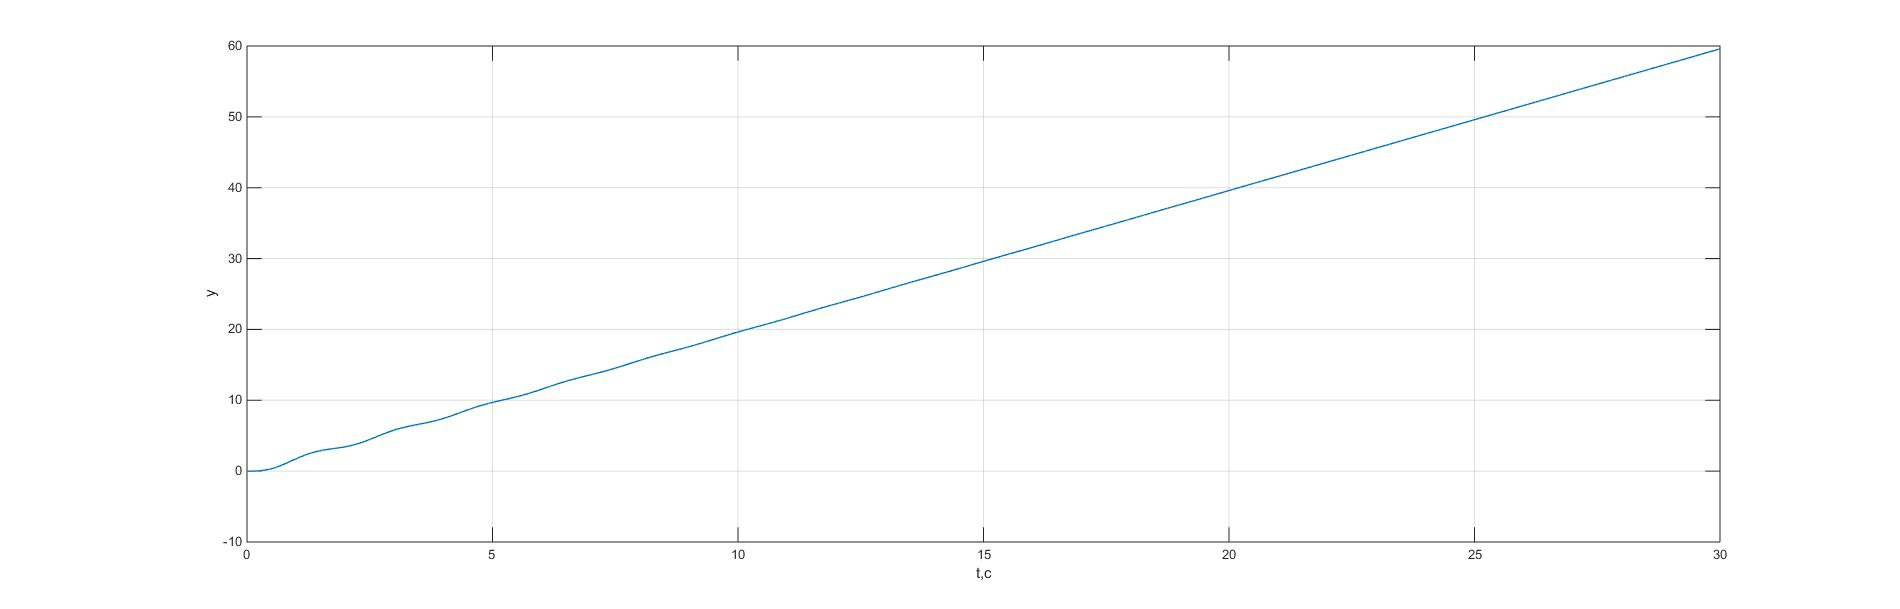
\includegraphics[width=1\linewidth]{2/21_y_k5_2t}}
    \caption{График переходного процесса при К=5}
    \label{two}
\end{figure}

\begin{figure}[h!]
    \center{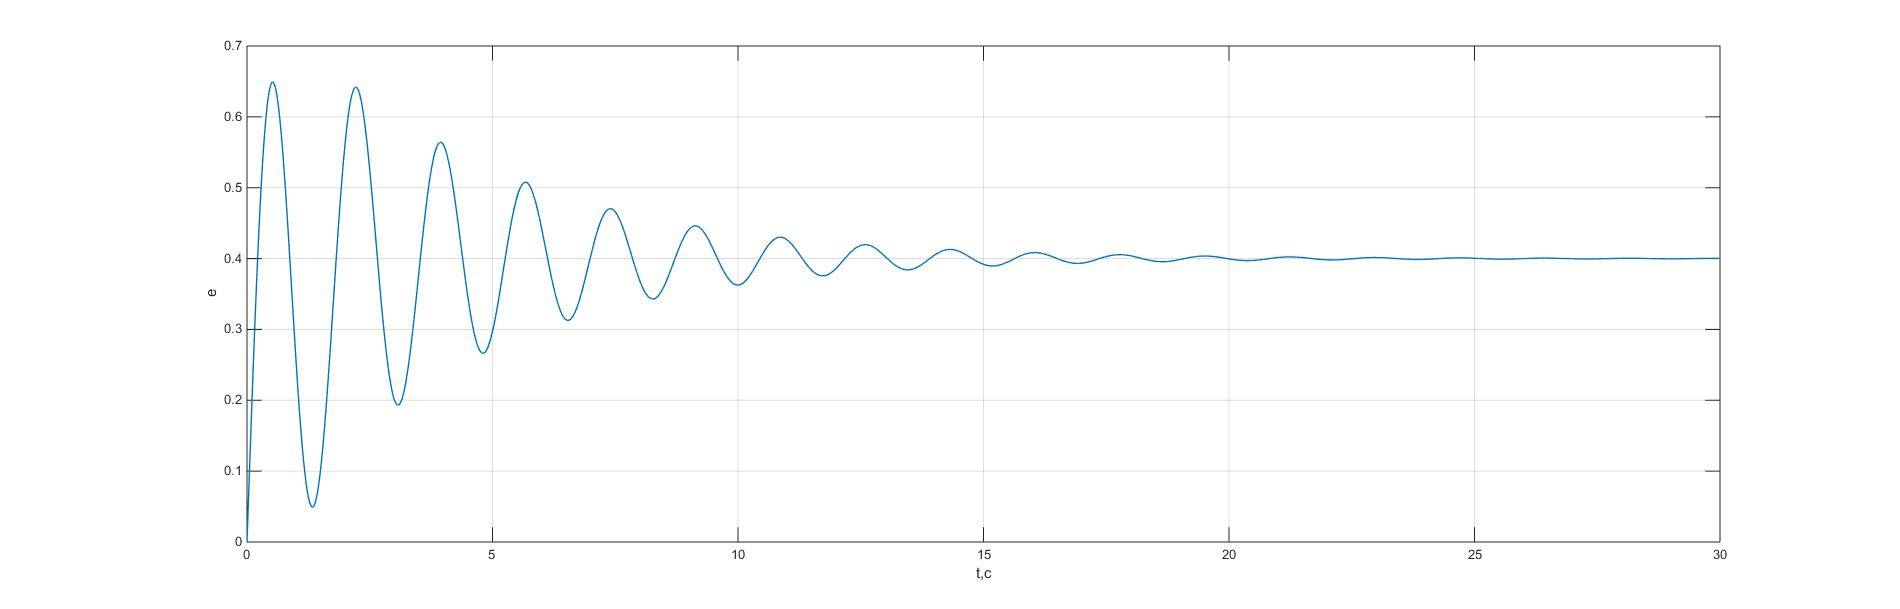
\includegraphics[width=1\linewidth]{2/22_e_k5_2t}}
    \caption{График ошибки переходного процесса при К=5}
    \label{tree}
\end{figure}

Из графика видно, что предельное значение установившейся ошибки $\epsilon_y(t)=0.4$. Это значение подтверждается аналитическим расчетом: $\epsilon_y(t)=\lim_{s\to0}\frac{s}{s+k}V=\frac{V}{k}=0.4$\\

Рассмотрим переходные процессы Y(t) и e(t) при К=10

\begin{figure}[h!]
    \center{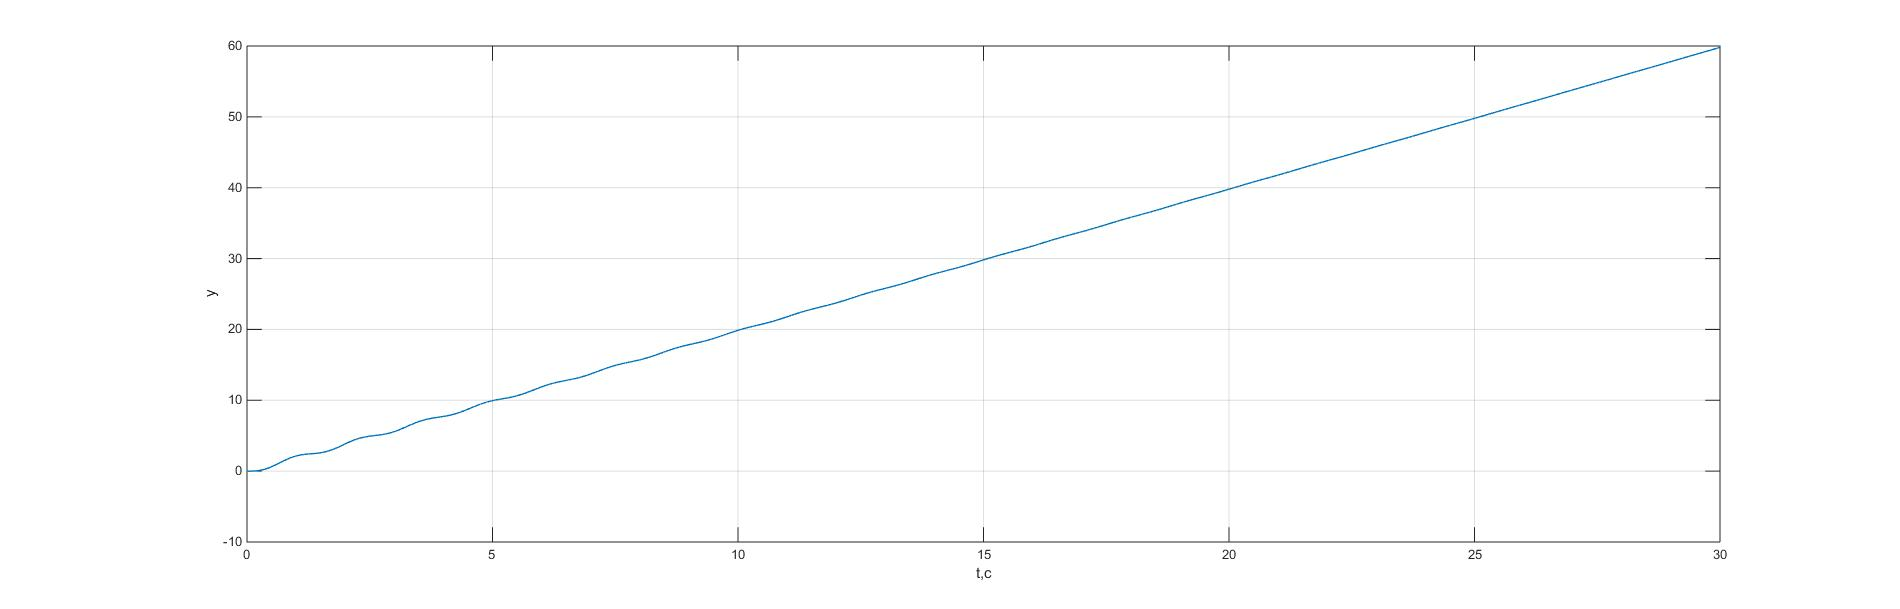
\includegraphics[width=1\linewidth]{2/23_y_k10_2t}}
    \caption{График переходного процесса при К=10}
    \label{two}
\end{figure}

\newpage

\begin{figure}[h!]
    \center{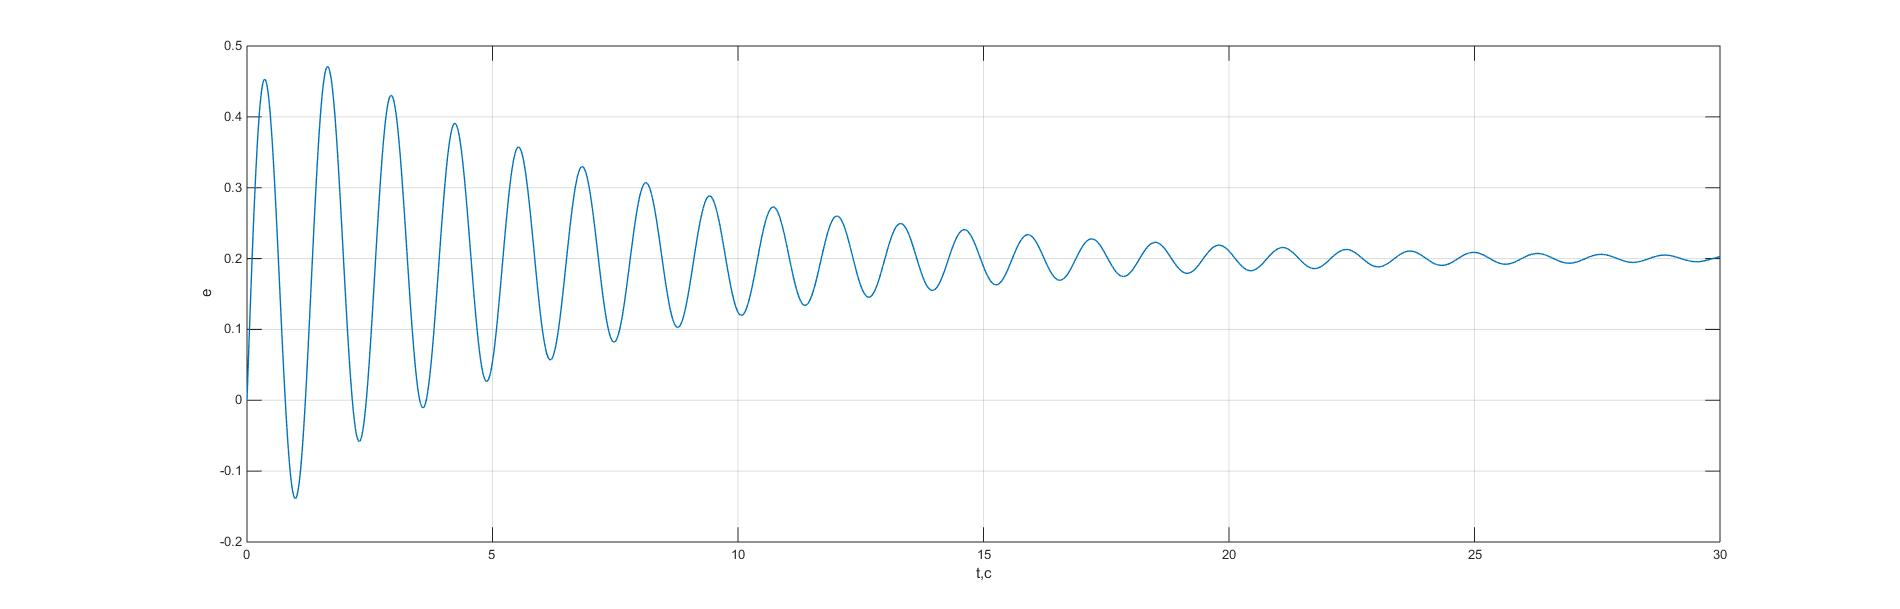
\includegraphics[width=1\linewidth]{2/24_e_k10_2t}}
    \caption{График ошибки переходного процесса при К=10}
    \label{tree}
\end{figure}

Из графика видно, что предельное значение установившейся ошибки $\epsilon_y(t)=0.2$. Это значение подтверждается аналитическим расчетом: $\epsilon_y(t)=\lim_{s\to0}\frac{s}{s+k}V=\frac{V}{k}=0.2$\\

\begin{table}[h]
    \begin{center}
    \begin{tabular}{|c|c|c|c|}
    \hline
         K & 1 & 5 & 10 \\
         \hline
         $\epsilon$ & 2 & 0.4 & 0.2 \\
    \hline     
    \end{tabular}
    \caption{Зависимость коэффициента от ошибки}
    \label{tab:my_label}
    \end{center}
\end{table}

\textbf{Вывод.} У системы управления (СУ) с первым порядком астатизма при линейно изменяющимся задающем воздействии (Vt) установившаяся ошибка равна $\epsilon=V/K$\\

%_______________В в параграфе 2

$g(t)=at^2/2$ – движение с постоянным ускорением.\\

Рассмотрим переходные процессы Y(t) и e(t) при К=1


\begin{figure}[h!]
    \center{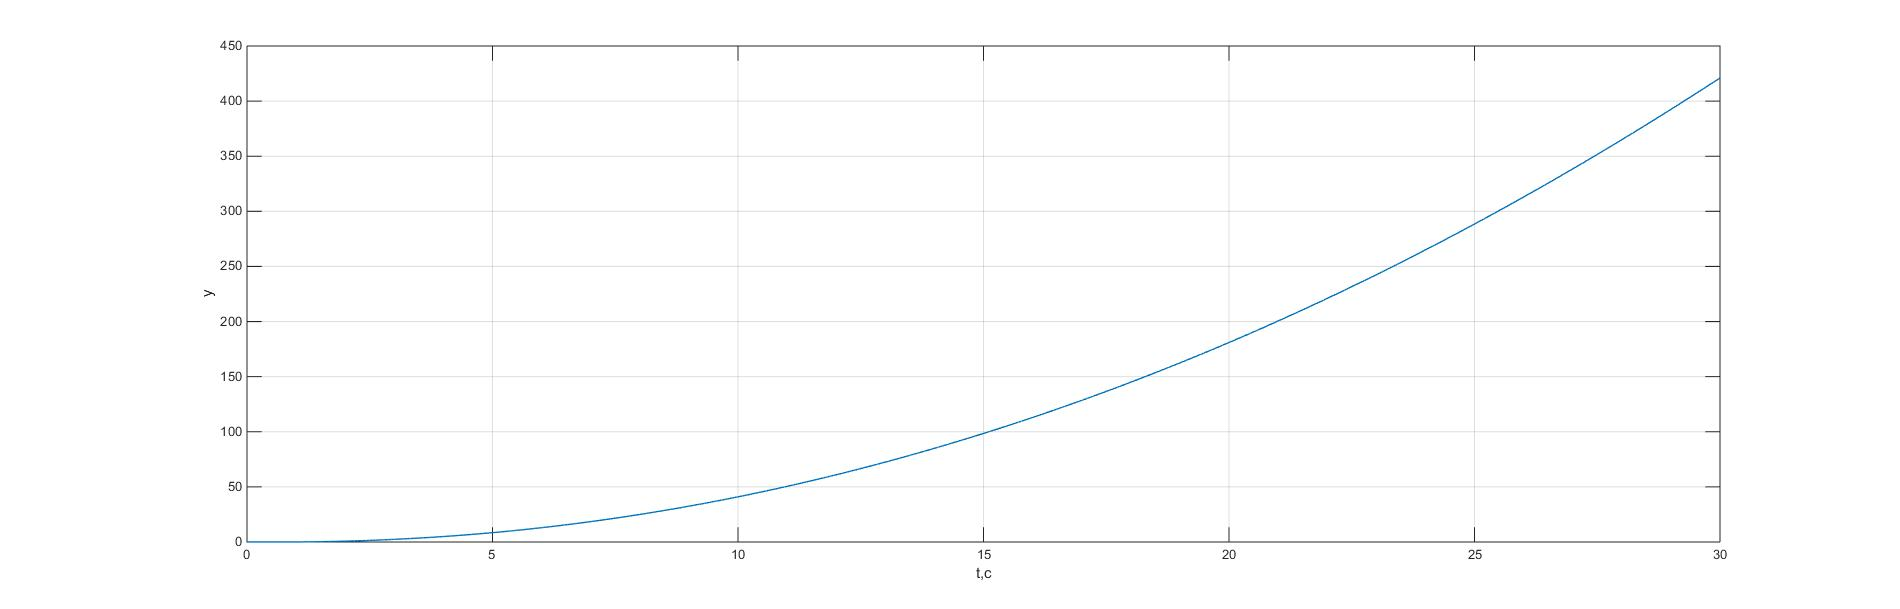
\includegraphics[width=1\linewidth]{2/25_y_k1_0,5t2}}
    \caption{График переходного процесса при К=1}
    \label{two}
\end{figure}

\newpage

\begin{figure}[h!]
    \center{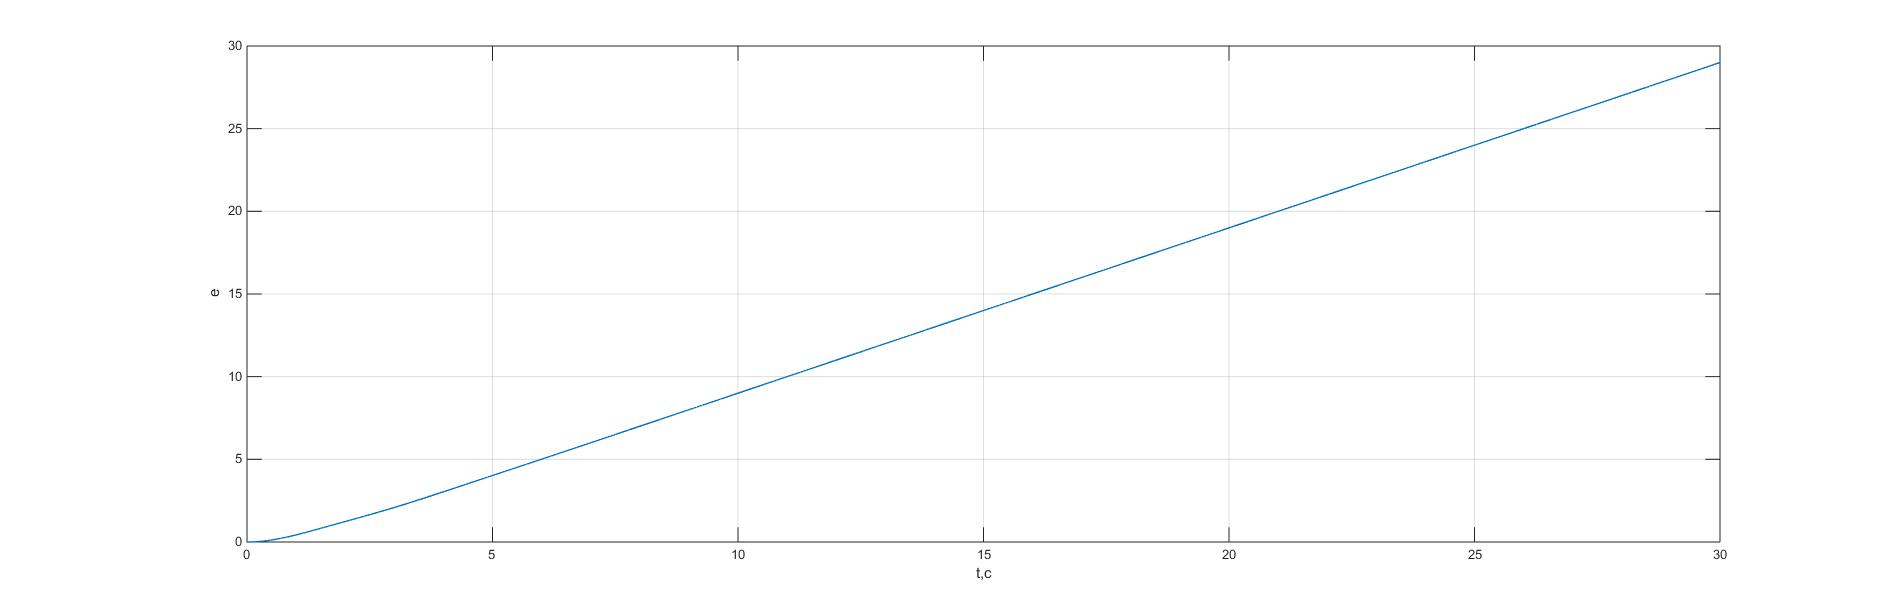
\includegraphics[width=1\linewidth]{2/26_e_k1_0,5t2}}
    \caption{График ошибки переходного процесса при К=1}
    \label{tree}
\end{figure}

Рассмотрим переходные процессы Y(t) и e(t) при К=5

\begin{figure}[h!]
    \center{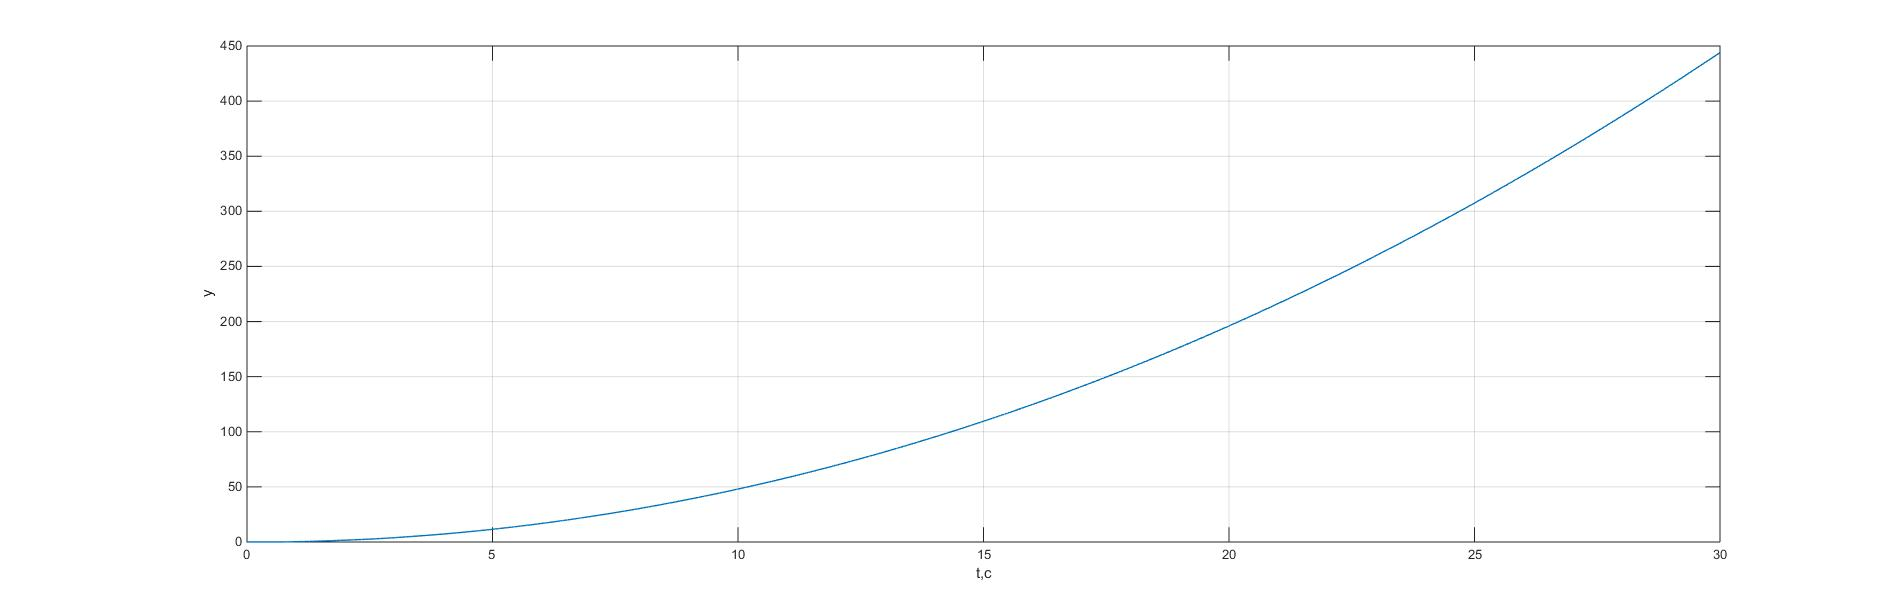
\includegraphics[width=1\linewidth]{2/27_y_k5_0,5t2}}
    \caption{График переходного процесса при К=5}
    \label{two}
\end{figure}

\begin{figure}[h!]
    \center{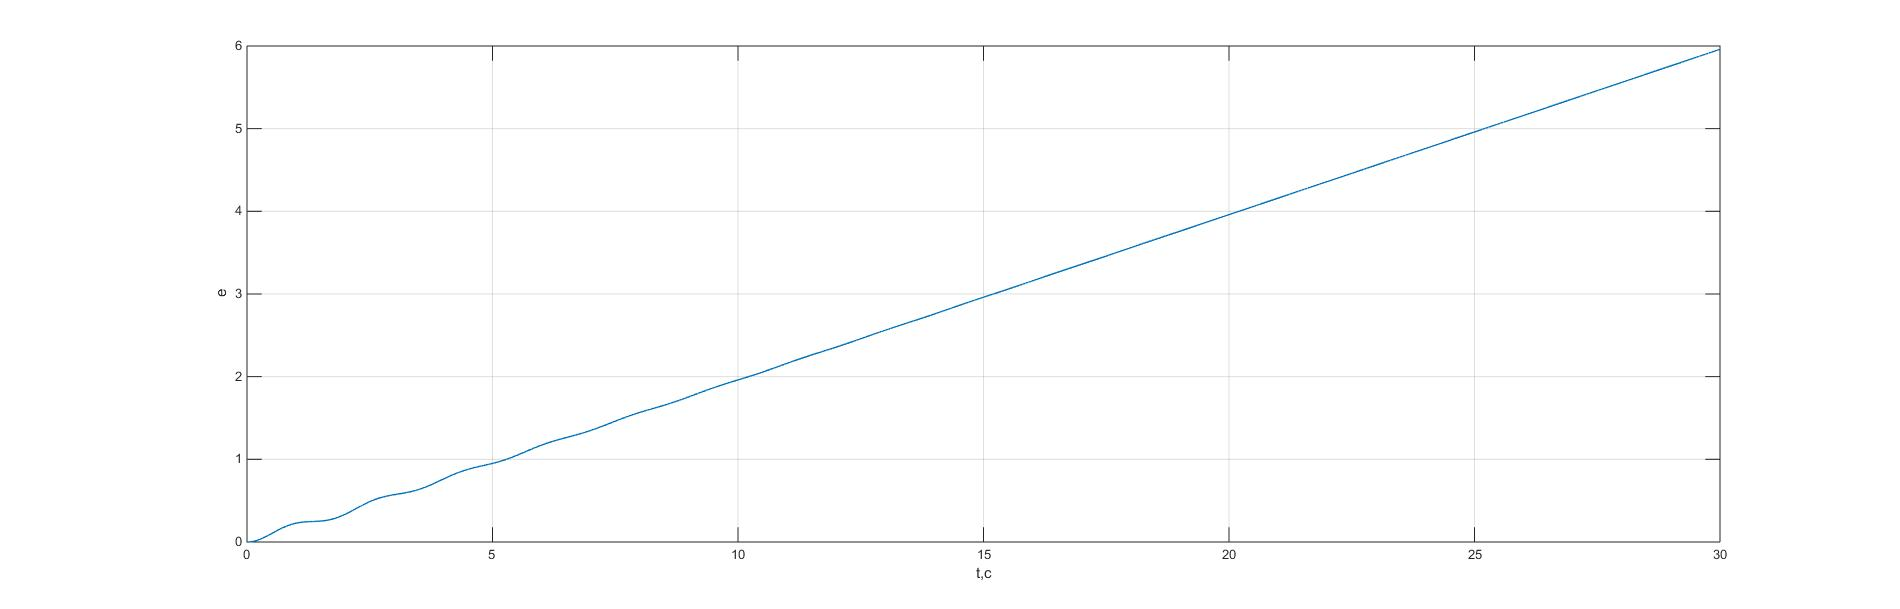
\includegraphics[width=1\linewidth]{2/28_e_k5_0,5t2}}
    \caption{График ошибки переходного процесса при К=5}
    \label{tree}
\end{figure}

\newpage

Рассмотрим переходные процессы Y(t) и e(t) при К=10

\begin{figure}[h!]
    \center{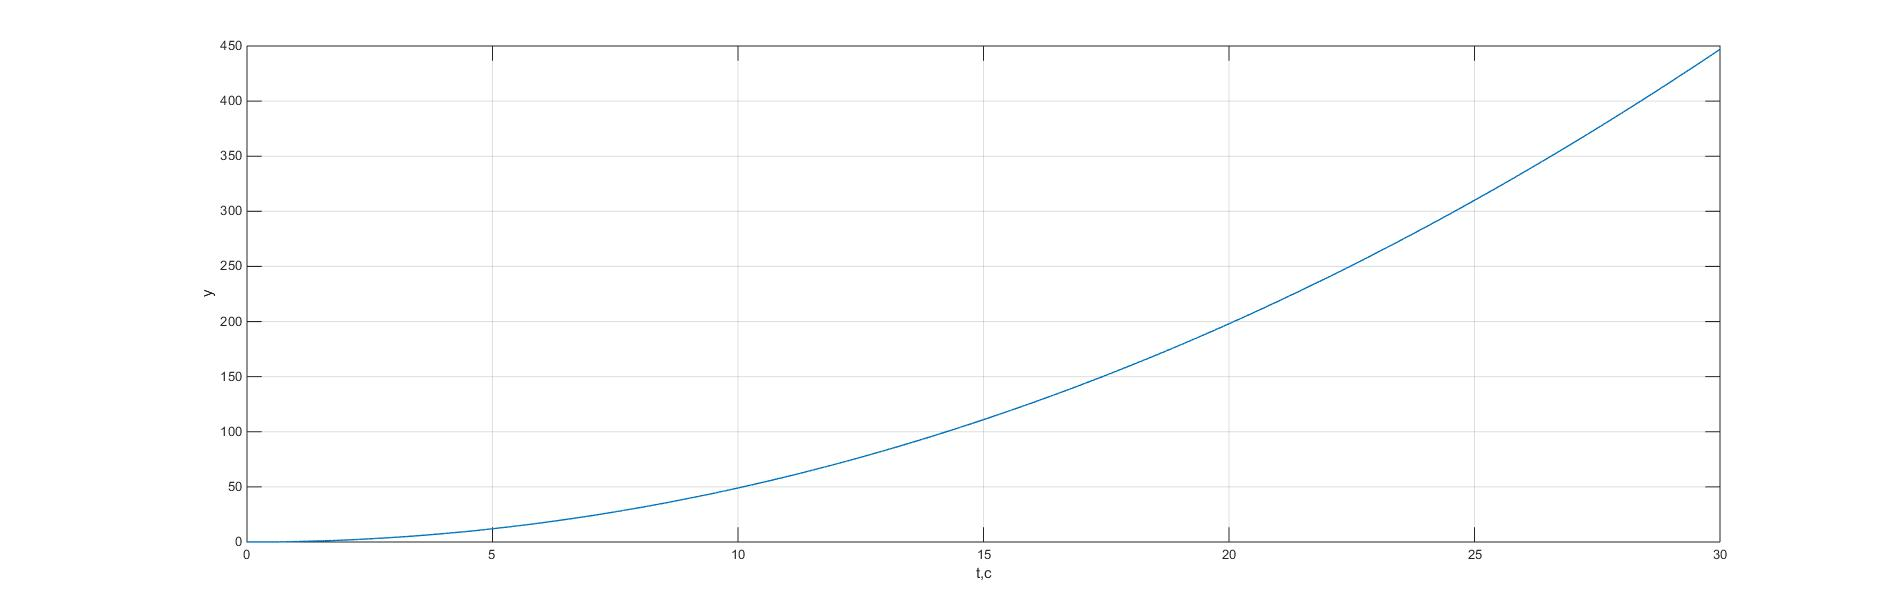
\includegraphics[width=1\linewidth]{2/29_y_k10_0,5t2}}
    \caption{График переходного процесса при К=10}
    \label{two}
\end{figure}

\begin{figure}[h!]
    \center{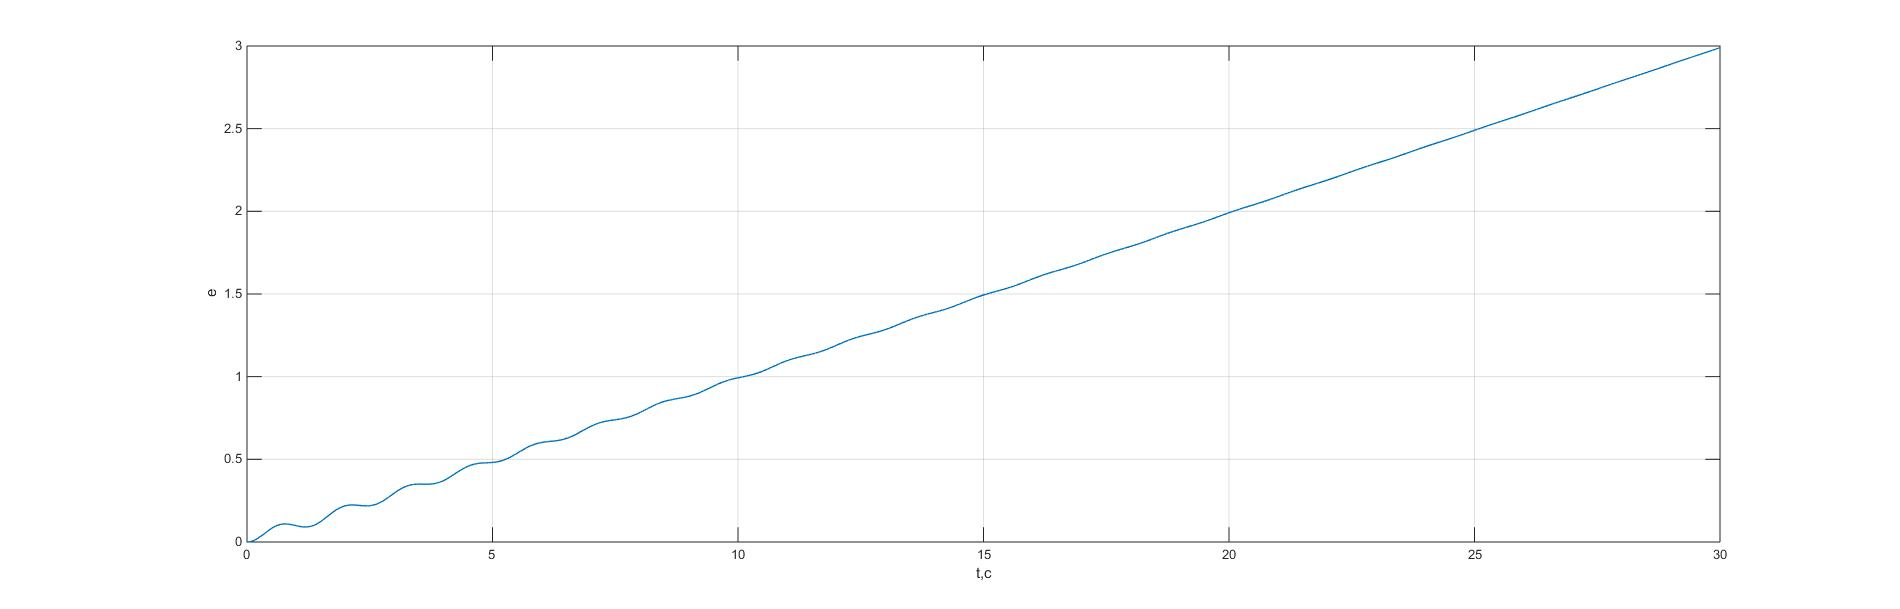
\includegraphics[width=1\linewidth]{2/30_e_k10_0,5t2}}
    \caption{График ошибки переходного процесса при К=10}
    \label{tree}
\end{figure}

\newpage
%ТРЕТИЙ ПАРАГРАФ______________!!!!!!!!!!!!!!!!!
\paragraph{Исследование влияния внешних возмущений.\\} $f_1=2,  f_2=0.5$

\begin{figure}[h]
    \center{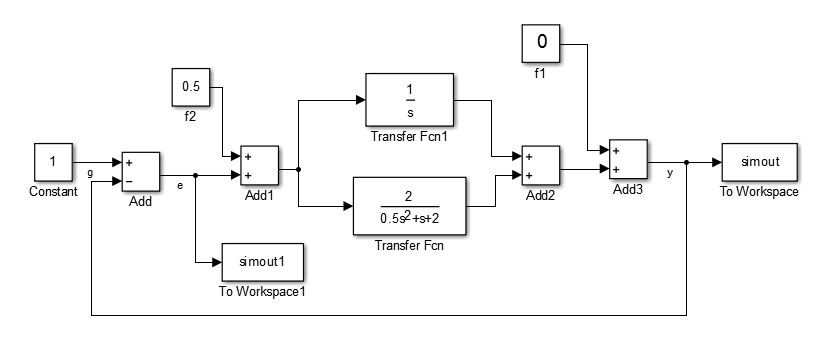
\includegraphics[width=1\linewidth]{3}}
    \caption{Схема моделирования влияния внешних возмущений.}
    \label{tree}
\end{figure}

Зададим $f_2(t) = 0, g(t) = 1(t)$

\begin{figure}[h!]
    \center{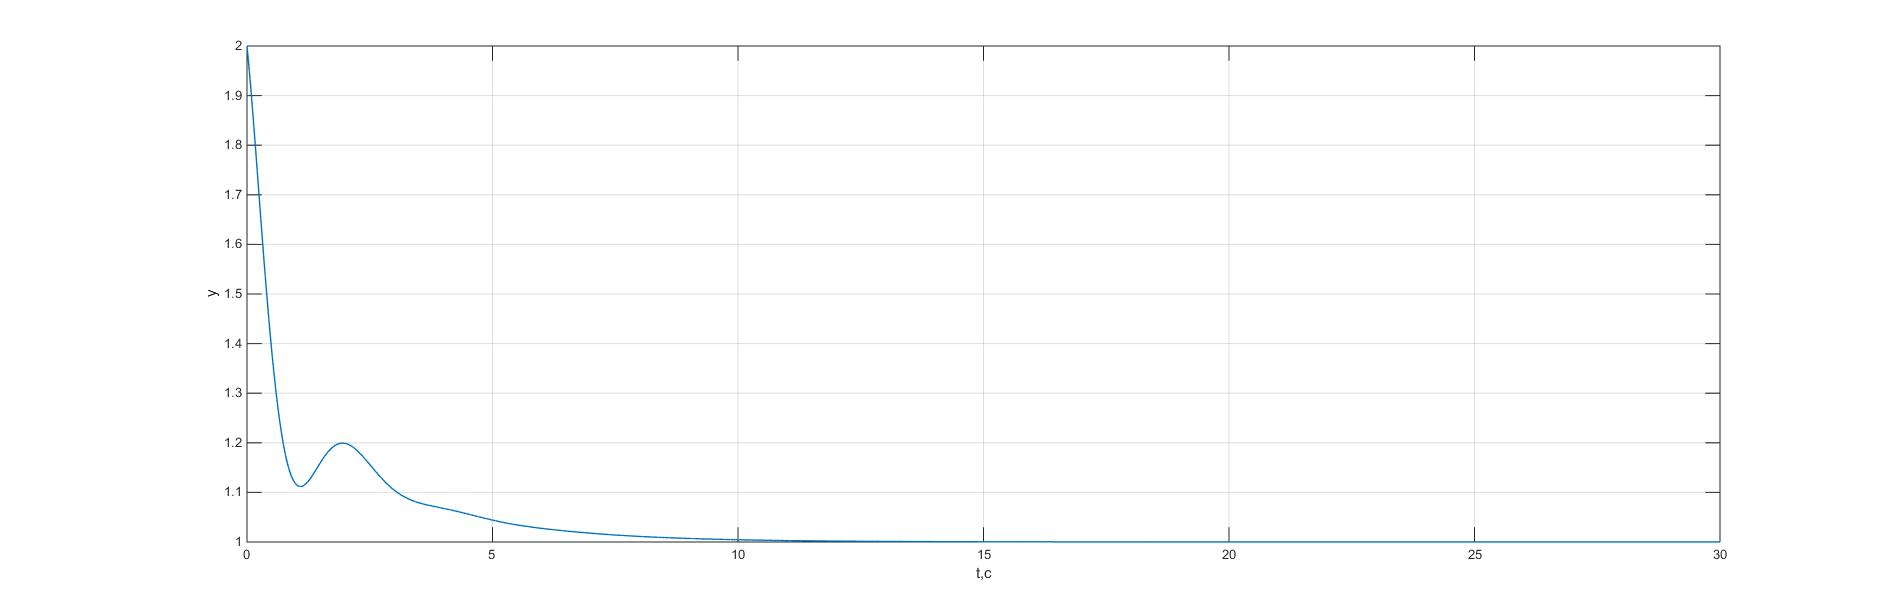
\includegraphics[width=1\linewidth]{3/31}}
    \caption{График переходного процесса при $f_2(t) = 0$}
    \label{two}
\end{figure}

\begin{figure}[h!]
    \center{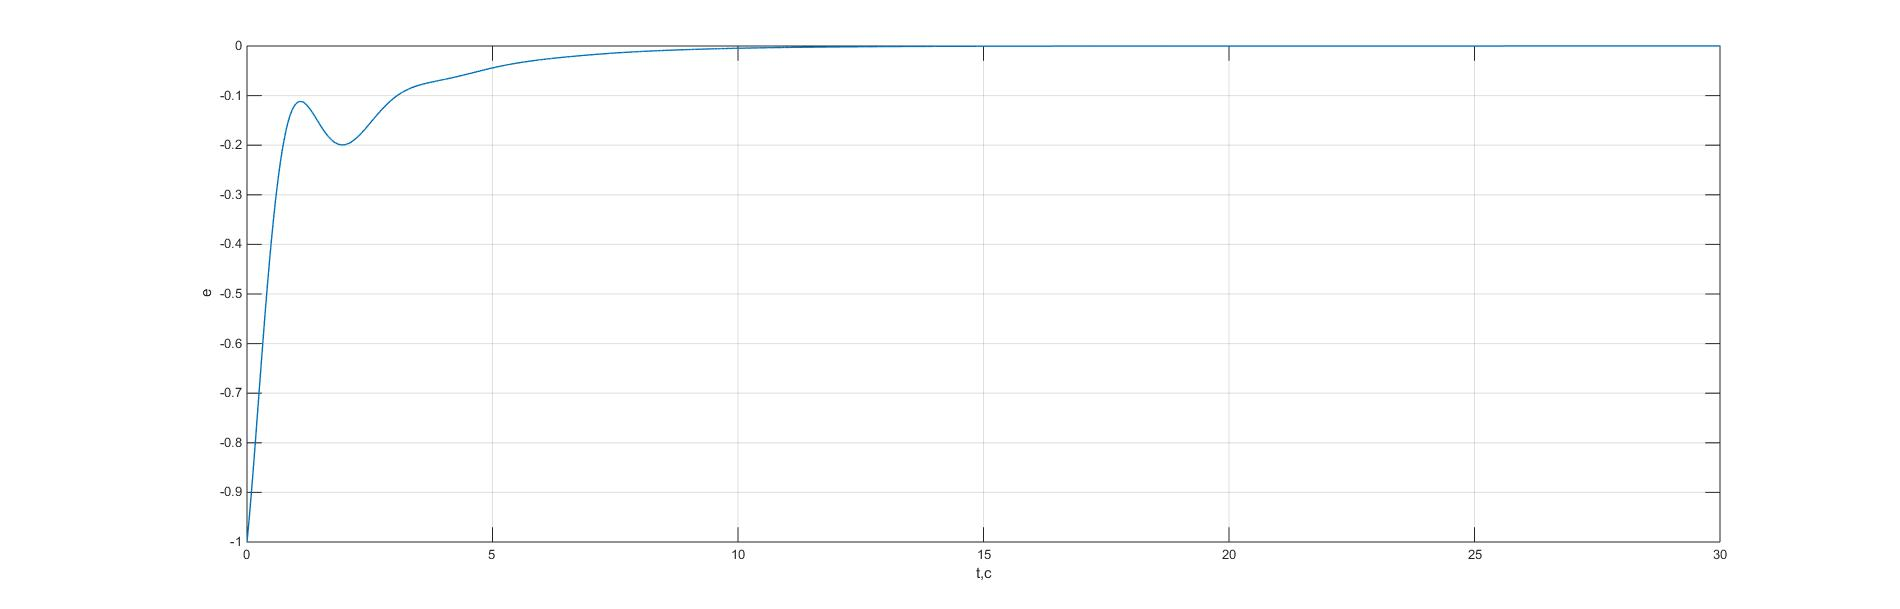
\includegraphics[width=1\linewidth]{3/32}}
    \caption{График ошибки переходного процесса при $f_2(t) = 0$}
    \label{tree}
\end{figure}

\newpage

Зададим $f_1(t) = 0, g(t) = 1(t)$

\begin{figure}[h]
    \center{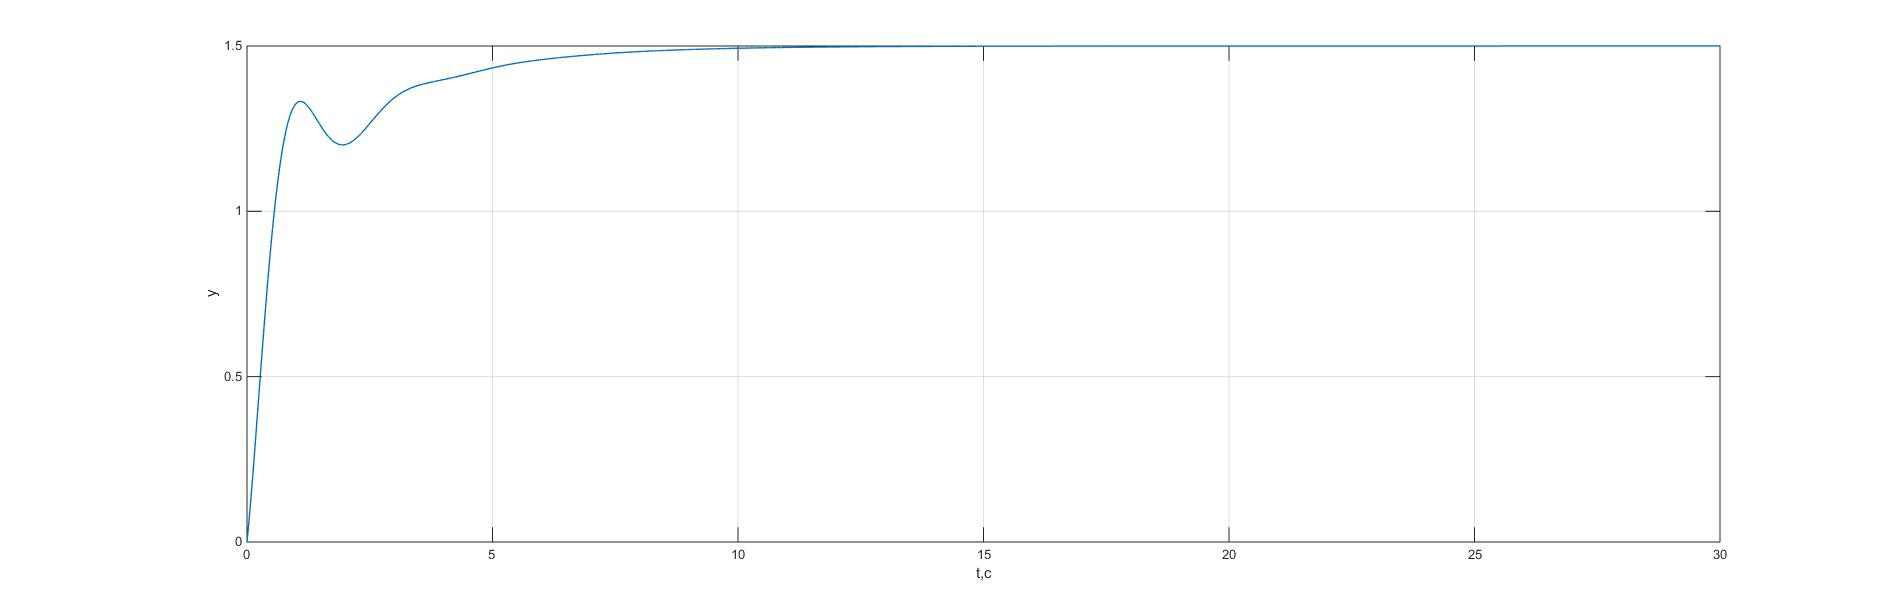
\includegraphics[width=1\linewidth]{3/33}}
    \caption{График переходного процесса.}
    \label{two}
\end{figure}
    
\begin{figure}[h]
    \center{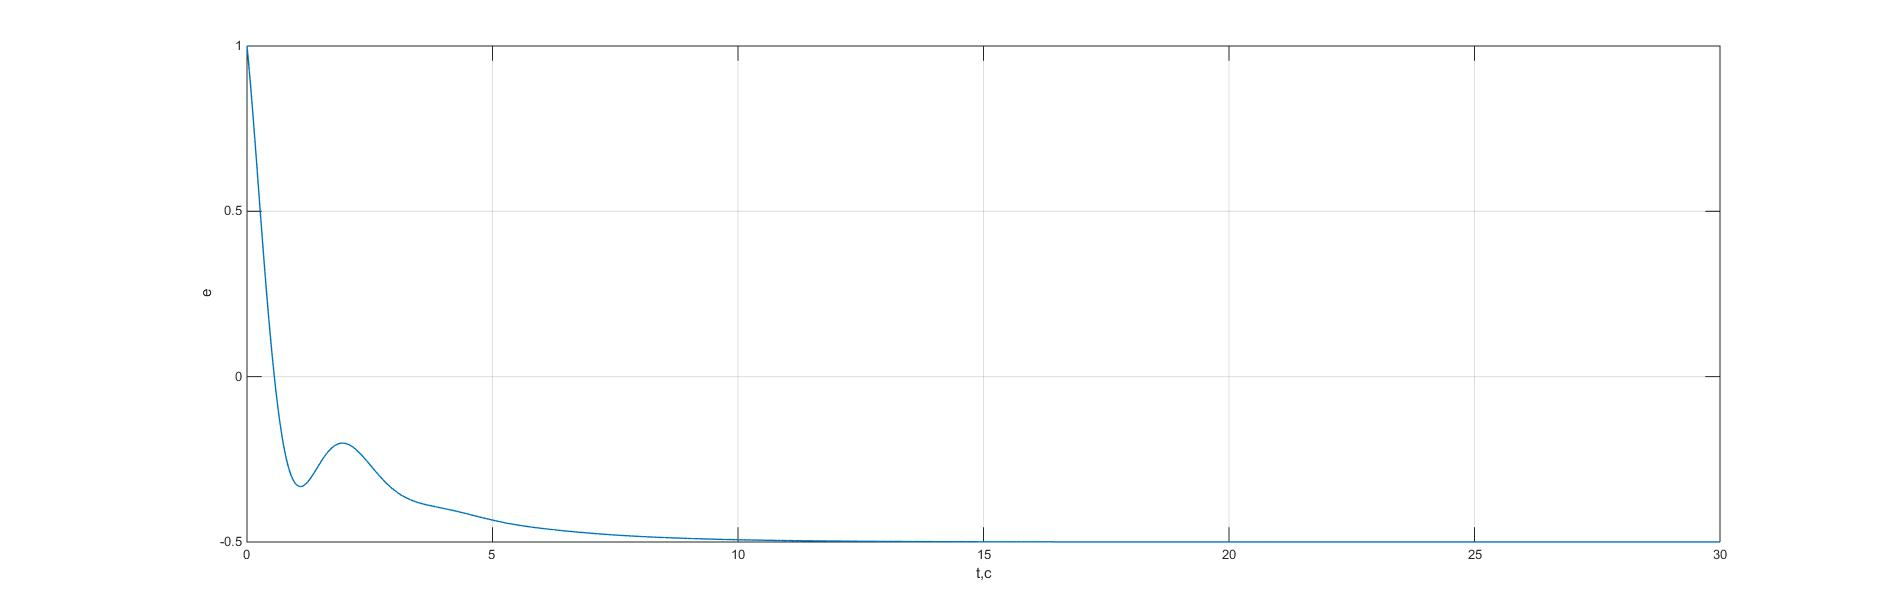
\includegraphics[width=1\linewidth]{3/34}}
    \caption{График ошибки переходного процесса.}
    \label{tree}
\end{figure}

Из графика видно, что предельное значение установившейся ошибки $e_y(t)=-0.5$. Это значение подтверждается аналитическим расчетом:
$e_y(t)=F_2=-0.5$
\newpage
\paragraph{Исследование установившейся ошибки при произвольном входном воздействии.} Рассмотрим систему при:\\
$H(s)=1; \\\\ 
W(s)=\frac {2} {0.5s^2+s+2}; \\\\  
g(t)=2+0.1t^2;$

\begin{figure}[h!]
    \center{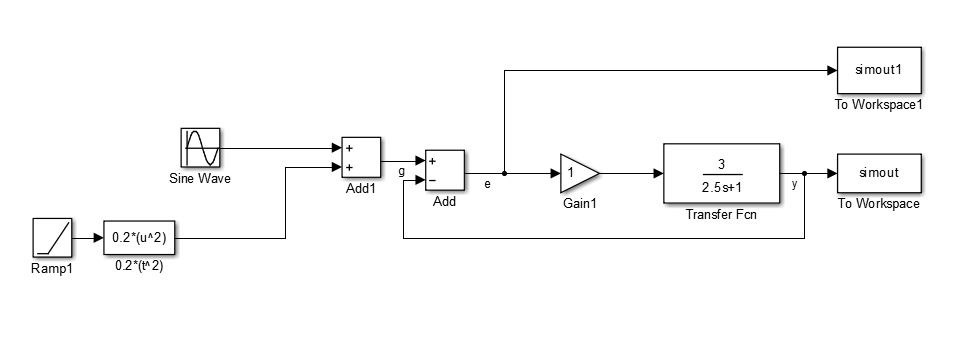
\includegraphics[width=1\linewidth]{4}}
    \caption{Схема моделирования произвольного входного воздействия.}
    \label{two}
\end{figure}

\begin{figure}[h!]
    \center{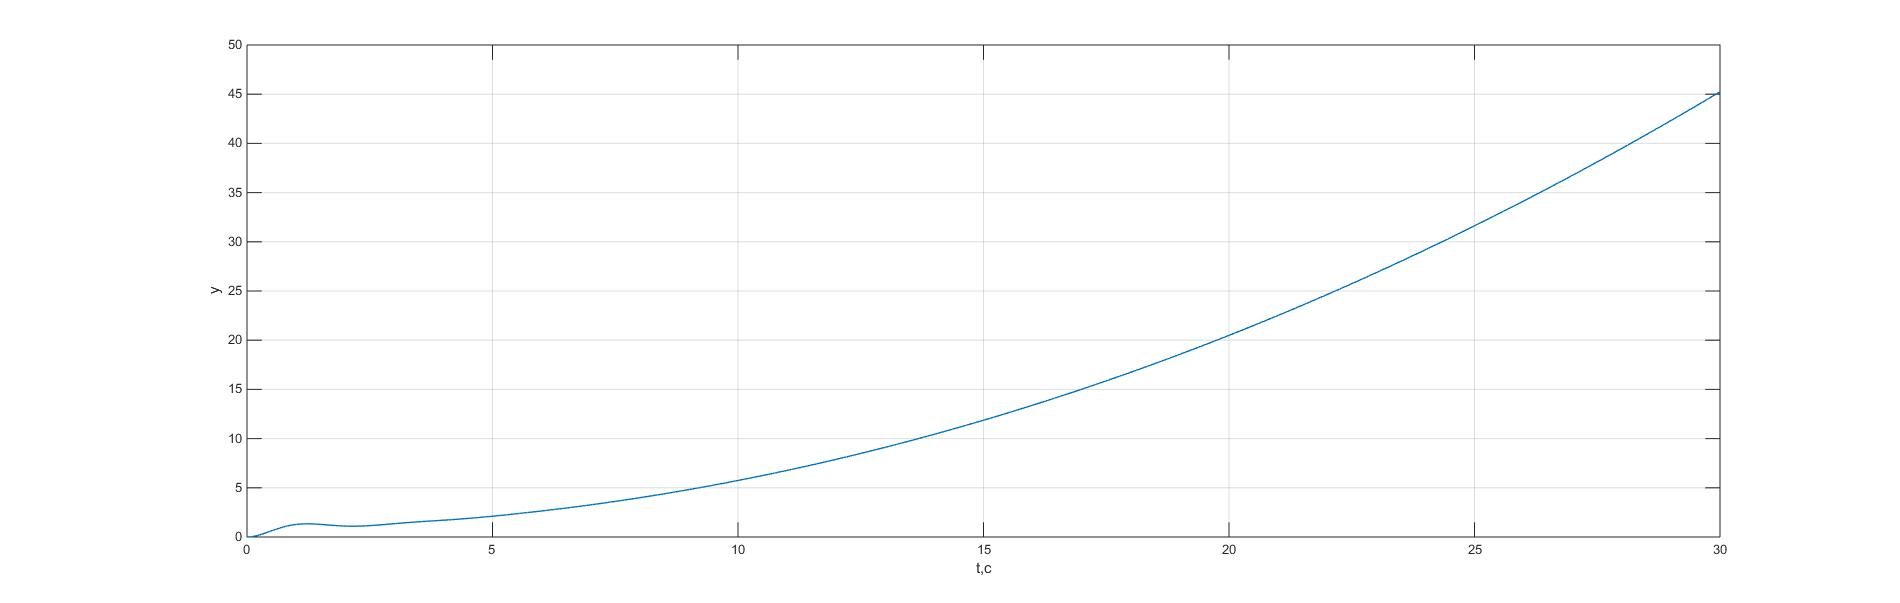
\includegraphics[width=1\linewidth]{4/35_y}}
    \caption{График переходного процесса.}
    \label{two}
\end{figure}
    
\begin{figure}[h!]
    \center{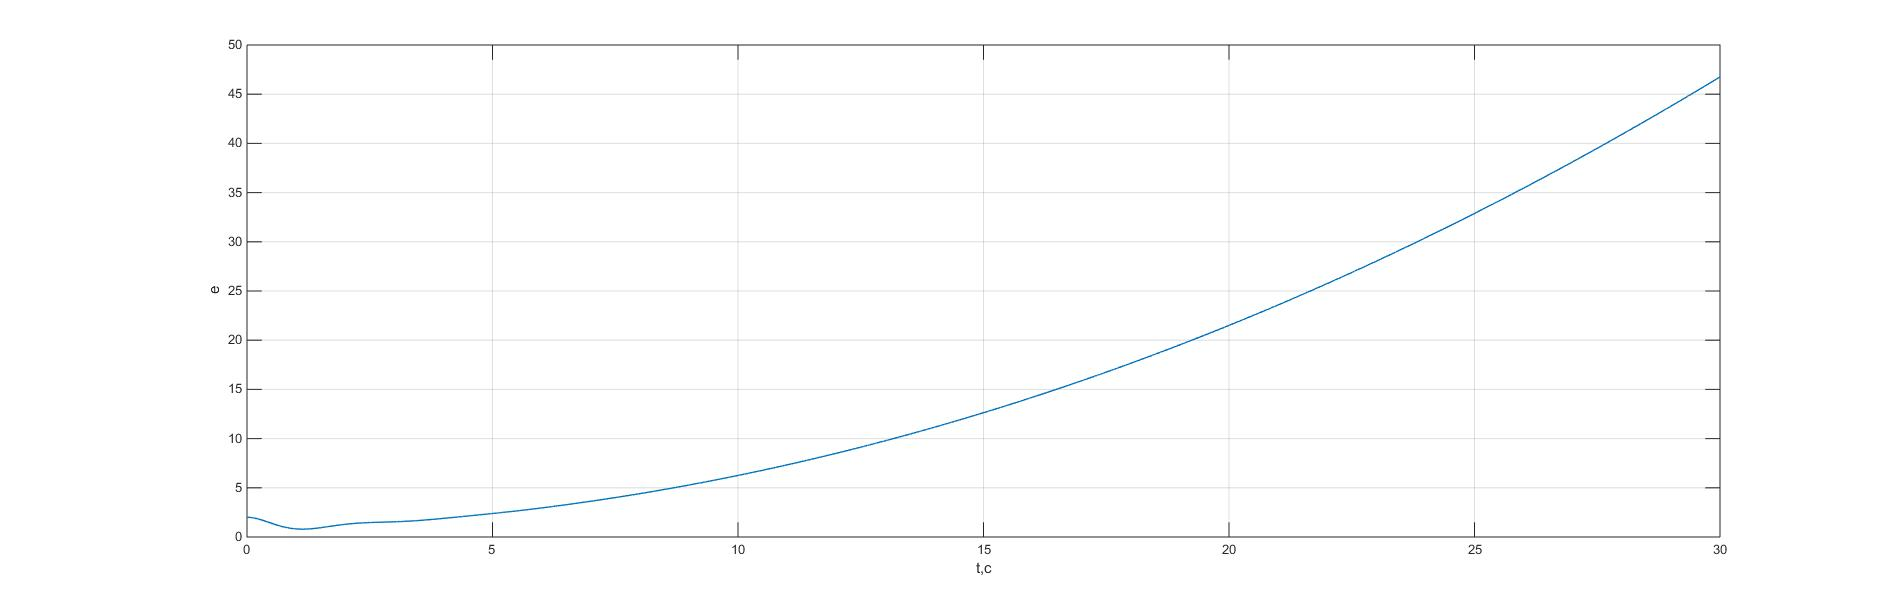
\includegraphics[width=1\linewidth]{4/36_e}}
    \caption{График ошибки переходного процесса.}
    \label{tree}
\end{figure}

\newpage

$e_y(t)\to\infty$, т.к. СУ с астатизмом нулевого порядка не может отработать линейно нарастающее задающее воздействие.\\

$e_y(t)=c_0g(t)+c_1\frac{d}{dt}g(t)+\frac{c_2}{2!}\frac{d^2}{dt^2}g(t)+...$ - где постоянные $c_i$ - коэффициенты ошибок.\\

$\Phi_e(s)=\frac{1}{1+W(s)}$, где W(s) – передаточная функция разомкнутой системы, Фe(s) – передаточная функция замкнутой системы по ошибке слежения (относительно задающего воздействия).\\
$W(s)=\frac {2} {0.5s^2+s+2}; \\\\
\Phi_e(s)=\frac{0.5s^2+s+2}{0.5s^2+s+4}$ \\\\
$c_0=\Phi_e(s) | _{s=0} =0.5 \\  c_1=0.125 \\ c_2=0.375$ \\\\
$e_y(t)=0.5(2+0.1t^2)+0.125*0.1t+0.125*0.1$

\begin{figure}[h]
    \center{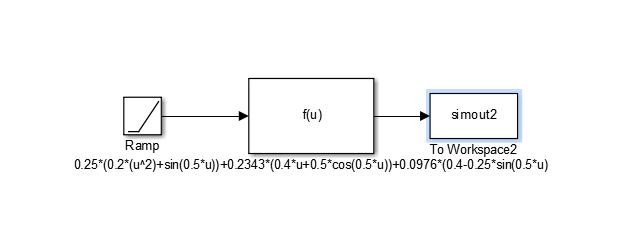
\includegraphics[width=1\linewidth]{teylor}}
    \caption{Схема моделирование. Ряд Тейлора.}
    \label{tree}
\end{figure}

\normalsize{При $t=0, e_s(t)=0.125$}

\begin{figure}[h]
    \center{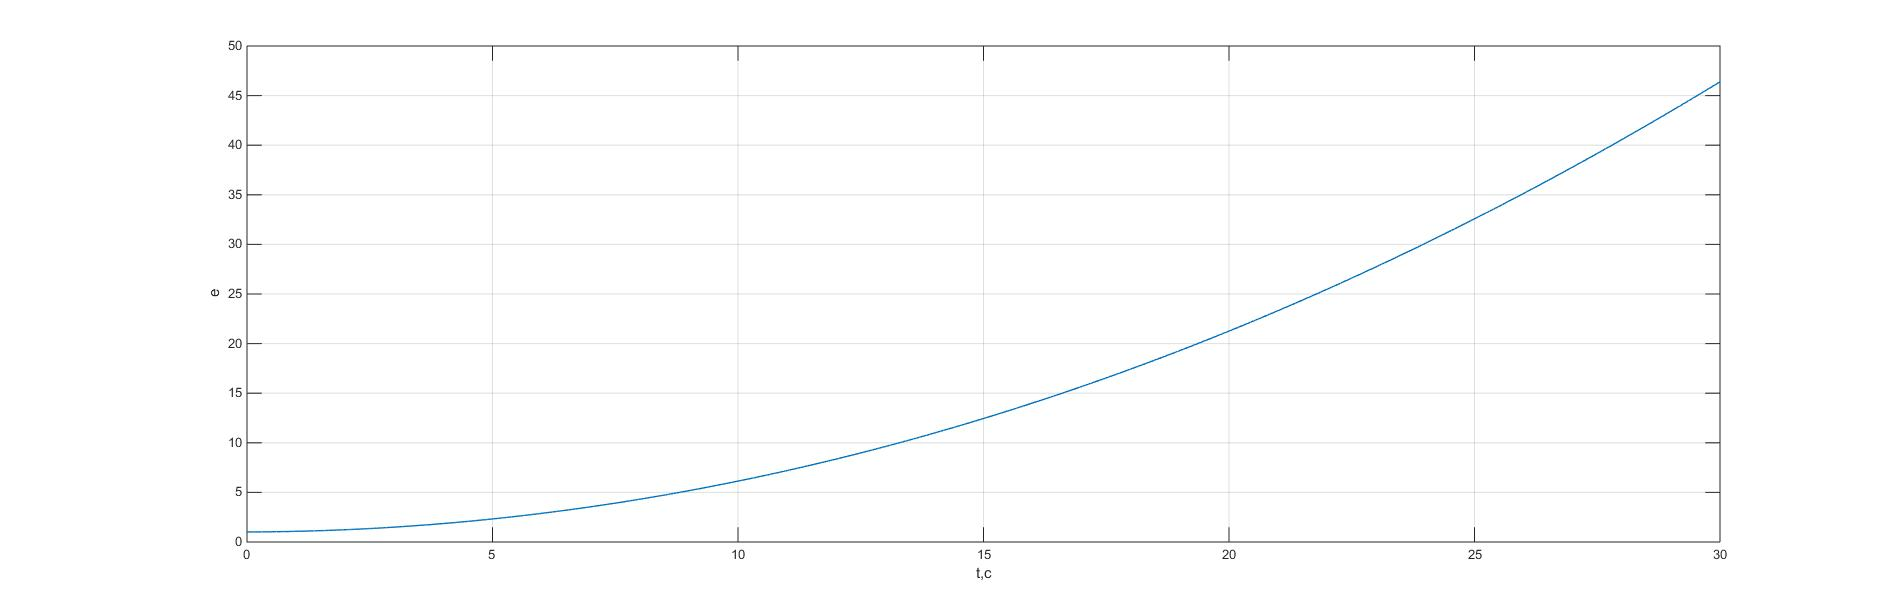
\includegraphics[width=1\linewidth]{4/37_e_teylor}}
    \caption{График ошибки переходного процесса.}
    \label{tree}
\end{figure}
\newpage
\paragraph{Вывод.} В данной работе мы по передаточной функции системы рассчитывали установившуюся ошибку системы и сравнивали ее со значением, полученным аналитически: результаты совпали. Проведенные нами исследования показали, что факт наличия или отсутствия установившейся ошибки должен быть определен для каждого действующего на систему возмущения на основе анализа соответствующих передаточных функций от возмущения к ошибке, вне зависимости от порядка астатизма системы по задающему воздействию.

\end{document} % КОНЕЦ ДОКУМЕНТА !

